\cleardoublepage\documentclass[../main.tex]{subfiles}
\begin{document}
\chapter{Aplicações das derivadas}\label{cap:apl_derivadas}\index{aplicações! derivadas}
\minitoc
%\tableofcontents
\subsection*{Objetivos de aprendizagem do capítulo}
\addcontentsline{toc}{section}{Objetivos de aprendizagem do capítulo}
Ao final deste capítulo você deverá ser capaz de:
\begin{itemize}
\item Aprender e Utilizar a regra de L’Hôpital para determinar os valores de limites indeterminados da forma \(0/0\), \(\infty/\infty\), \(\infty\cdot 0\), \(\infty-\infty\), \(1^\infty\), \(0^0\) e \(\infty^0\); 
\item Conhecer o Teorema de Valor Médio e suas generalizações;
\item Determinar os valores extremos, se existirem, de uma função dada;
    \item Determinar os pontos de inflexão, se existirem, e os intervalos de concavidade para cima e concavidade para baixo de uma função dada;
    \item Estabelecer se uma função é crescente ou decrescente em um intervalo;
    \item Esboçar gráficos de funções;
    \item Resolver problemas de taxas de variação e otimização que envolvem conceitos de derivadas.
\end{itemize}

\section{Introdução}
Neste capítulo, estudaremos várias aplicações da derivada. Começaremos com a \hyperlink{sec:lopital}{Regra de L’Hôpital} para calcular tipos específicos de limites indeterminados, o que é muito útil para resolver limites mais complexos que recaem em indeterminação e cujas expressões não são facilmente fatoráveis.

 Na Seção \ref{sec:diferencial} apresentamos aplicação relacionada ao conceito de diferencial de uma função. O Teorema do Valor Médio é apresentado na Seção \ref{sec:TVM}, o qual é útil quando queremos garantir a existência
de determinados pontos com certas propriedades envolvendo a derivada.

 Outras aplicações importantes estão relacionadas ao cálculo de extremos de funções (\autoref{sec:extremosFunc}) e crescimento e decrescimento de funções (\autoref{sec:FuncCrescDecresc}). Cálculo de valores máximos e mínimos de funções é uma outra aplicação de derivadas, exibida na seção  \ref{sec:MaxMin}. Na Seção \ref{sec:taxaVariac} são apresentadas aplicações das derivadas relacionada a taxas de variação, que subsidia na resolução de diversos problemas em diferentes áreas do conhecimento. Por fim, na Seção \ref{sec:Otmiz}, são apresentados problemas de otimização.

No apêndice \ref{apend:MetNewton} são apresentadas mais aplicações de derivadas.

\section{Regra de L'Hôpital}\hypertarget{Lopital}{}\label{sec:lopital}
A \hypertarget{sec:lopital}{regra de L'Hôpital} é uma técnica para o cálculo de limites de indeterminações. Sejam $f$ e $g$ funções deriváveis em um intervalo aberto contendo $x=a$, exceto possivelmente em $x=a$, e
\begin{equation}
  \lim_{x\to a} f(x) = 0\quad\text{e}\quad\lim_{x\to a} g(x) = 0
\end{equation}
Se, ainda, $\lim_{x\to a} f(x)/g(x)$ existe ou for $\pm\infty$, então
\begin{equation}
  \lim_{x\to a} \frac{f(x)}{g(x)} = \lim_{x\to a} \frac{f'(x)}{g'(x)}
\end{equation}
Esta é a versão da regra de L'Hôpital para indeterminações do tipo $0/0$. Sem grandes modificações, é diretamente estendida para os casos $x\to a^-$, $x\to a^+$, $x\to \infty$ e $x\to -\infty$.\\

\nota{A regra de L'Hôpital pode ser aplicada repetidas vezes enquanto a indeterminação se manter.\\
%Em tratamentos mais avançados de cálculo é provado que a regra de L’Hôpital aplica-se à forma indeterminada \(\infty/\infty\), da mesma forma que \(0/0\), ou seja, se \(f(x)\to \pm\infty\) e \(g(x)\to \pm\infty\), quando \(x\to a\), então
%\[ \lim \limits_{x\to a}\dfrac{f(x)}{g(x)}= \lim \limits_{x\to a}\dfrac{f'(x)}{g'(x)}. \]
}
\begin{ex}
  Vamos calcular o limite
  \begin{equation*}
    \lim_{x\to 1} \frac{x-1}{x^2-1}
  \end{equation*}
  \begin{enumerate}[a)]
  \item Pela regra de L'Hôpital.
    \begin{align*}
      \lim_{x\to 1} \frac{x-1}{x^2-1} &= \lim_{x\to 1} \frac{(x+1)'}{(x^2-1)'} \\
                                      &= \lim_{x\to 1} \frac{1}{2x} \\
                                      &= \frac{1}{2}
    \end{align*}
  \item Por eliminação do fator comum.
    \begin{align*}
      \lim_{x\to 1} \frac{x-1}{x^2-1} &= \lim_{x\to 1} \frac{x-1}{(x-1)(x+1)} \\
                                      &= \lim_{x\to 1} \frac{1}{x+1} \\
                                      &= \frac{1}{2}
    \end{align*}
  \end{enumerate}
 \end{ex}

\begin{ex}
  O limite
  \begin{equation}
    \lim_{x\to 2} \frac{x^2-4x+4}{x^3-3x^2+4}
  \end{equation}
  é uma indeterminação $0/0$. Aplicando a regra de L'Hôpital, obtemos
  \begin{equation*}
    \lim_{x\to 2} \frac{x^2-4x+4}{x^3-3x^2+4} = \lim_{x\to 2} \frac{\cancelto{0}{2x-4}}{\cancelto{0}{3x^2-6x}}
  \end{equation*}
  que também é uma indeterminação do tipo $0/0$. Agora, aplicando a regra de L'Hôpital novamente, obtemos
  \begin{equation*}
    \lim_{x\to 2} \frac{2x-4}{3x^2-6x} = \lim_{x\to 2} \frac{2}{6x-6} = \frac{1}{3}
  \end{equation*}
  Portanto, concluímos que
  \begin{equation*}
    \lim_{x\to 2} \frac{x^2-4x+4}{x^3-3x^2+4} = \frac{1}{3}
  \end{equation*}  
\end{ex}

\begin{obs}
  A regra de L'Hôpital também pode ser usada para indeterminações do tipo $\infty/\infty$.
\end{obs}

\begin{ex}
  Vamos calcular
  \begin{equation*}
    \lim_{x\to \infty} \frac{e^x}{x}
  \end{equation*}
  que é uma indeterminação do tipo $\infty/\infty$. Então, aplicando a regra de L'Hôpital, temos
  \begin{equation*}
    \lim_{x\to \infty} \frac{e^x}{x} = \lim_{x\to \infty} \frac{e^x}{1} = \infty
  \end{equation*}
\end{ex}

\addcontentsline{toc}{subsection}{Exercícios resolvidos}
%\subsection{Exercícios resolvidos}
\subsubsection*{\emph{Caso I: Indeterminação do tipo} $\mathbf{0/0}$}
\begin{exeresol}
  Calcule
  \begin{compactenum}[a)]
   \item \(\lim \limits_{x\to 0}\dfrac{1-e^{2x}}{x}\)\\
  
  \begin{resol}
  Fazendo \(f(x)=1-e^{2x}\) e \(g(x)=x\), temos que

\[ \lim \limits_{x\to 0}f(x)=0 \quad \mbox{e}\quad \lim \limits_{x\to 0}g(x)=0. \]
Logo, podemos aplicar a regra de L’Hôpital. Das definições de \(f(x)\) e \(g(x)\), temos que \(f'(x)=-2e^{2x}\) e \(g'(x)=1\). Assim,
\[ \lim \limits_{x\to 0}\dfrac{1-e^{2x}}{x}=\lim \limits_{x\to 0}\dfrac{(1-e^{2x})'}{(x)'}=\lim \limits_{x\to 0}\dfrac{-2e^{2x}}{1}=-2. \]
Portanto, \(\lim \limits_{x\to 0}\dfrac{1-e^{2x}}{x}=-2\).
  \end{resol}
  \item \(\lim \limits_{x\to 0}\dfrac{{\rm sen}(x)}{x}\)\\
  
  \begin{resol}
  Fazendo \(f(x)={\rm sen}(x)\) e \(g(x)=x\), temos que

\[ \lim \limits_{x\to 0}f(x)=0 \quad \mbox{e}\quad \lim \limits_{x\to 0}g(x)=0. \]
Logo, podemos aplicar a regra de L’Hôpital. Das definições de \(f(x)\) e \(g(x)\), temos que \(f'(x)=\cos(x)\) e \(g'(x)=1\). Assim

\[ \lim \limits_{x\to 0}\dfrac{{\rm sen}(x)}{x}=\lim \limits_{x\to 0}\dfrac{({\rm sen}(x))'}{(x)'}=\lim \limits_{x\to 0}\dfrac{\cos(x)}{1}=1. \]
Portanto, \(\lim \limits_{x\to 0}\dfrac{{\rm sen}(x)}{x}=1\).
  \end{resol}
   \item \( \lim_{x\to 0^-} \frac{e^x-1}{x^2}\)\\
  
  \begin{resol}
   Observamos tratar-se de uma indeterminação do tipo $0/0$, i.e.
  \begin{equation*}
    \lim_{x\to 0^-} \frac{\cancelto{0}{e^x-1}}{\cancelto{0}{x^2}}
  \end{equation*}
  Então, aplicando a regra de L'Hôpital, temos
  \begin{equation*}
    \lim_{x\to 0^-} \frac{e^x-1}{x^2} = \lim_{x\to 0^-} \frac{\cancelto{1}{e^x}}{\cancelto{0^-}{2x}} = -\infty
  \end{equation*}
  \end{resol}
  \item \(\lim \limits_{x\to 0}\dfrac{x-{\rm tg}(x)}{x-{\rm sen}(x)}\)\\
  
  \begin{resol}
  Fazendo \(f(x)=x-{\rm tg}(x)\) e \(g(x)=x-{\rm sen}(x)\), temos que

\[ \lim \limits_{x\to 0}f(x)=0 \quad \mbox{e}\quad \lim \limits_{x\to 0}g(x)=0. \]
Logo, podemos aplicar a regra de L’Hôpital. Das definições de \(f(x)\) e \(g(x)\), temos que \(f'(x)=1-{\rm sec}^2(x)\) e \(g'(x)=1-\cos(x)\). Porém,

\[ \lim \limits_{x\to 0}f'(x)=0 \quad \mbox{e}\quad \lim \limits_{x\to 0}g'(x)=0 \]
Desde que o quociente das derivadas \(\dfrac{f'(x)}{g'(x)}\) tende à forma indeterminada \(0/0\), da Nota anterior, podemos aplicar a regra de L’Hôpital repetidas vezes até eliminar essa indeterminação. Neste caso, aplicaremos duas vezes mais a regra de L’Hôpital, ou seja, até a derivada de ordem \(3\). Assim

\[ \begin{array}{rcl} \lim \limits_{x\to 0}\dfrac{x-{\rm tg}(x)}{x-{\rm sen}(x)}&=&\lim \limits_{x\to 0}\dfrac{(x-{\rm tg}(x))'}{(x-{\rm sen}(x))'}=\lim \limits_{x\to 0}\dfrac{1-{\rm sec}^2(x)}{1-\cos(x)}\\\\ \lim \limits_{x\to 0}\dfrac{1-{\rm sec}^2(x)}{1-\cos(x)}&=&\lim \limits_{x\to 0}\dfrac{(1-{\rm sec}^2(x))'}{(1-\cos(x))'}=\lim \limits_{x\to 0}\dfrac{-2{\rm tg}(x){\rm sec}^2(x)}{{\rm sen}(x)} \\\\ \lim \limits_{x\to 0}\dfrac{-2{\rm tg}(x){\rm sec}^2(x)}{{\rm sen}(x)}&=&\lim \limits_{x\to 0}\dfrac{(-2{\rm tg}(x){\rm sec}^2(x))'}{({\rm sen}(x))'}=\lim \limits_{x\to 0}\dfrac{-2(1+3{\rm tg}^2(x))}{\cos^2(x)}=-2. \end{array} \]
Portanto, \(\,\,\lim \limits_{x\to 0}\dfrac{x-{\rm tg}(x)}{x-{\rm sen}(x)}=-2\).
  \end{resol}
   
  \end{compactenum}
  \end{exeresol}

\subsubsection*{\textbf{Caso II: Indeterminação do tipo} $\mathbf{\infty/\infty}$}
\begin{exeresol}
  \begin{compactenum}[a)]
  \item \(\lim \limits_{x\to +\infty}\dfrac{e^x}{x^2}\)
  
  \begin{resol}
  Desde que \(\lim \limits_{x\to \infty}e^x=\infty\) e \(\lim \limits_{x\to \infty}{x^2}=\infty\), obtemos

\[ \lim \limits_{x\to +\infty}\dfrac{e^x}{x^2}=\lim \limits_{x\to +\infty}\dfrac{(e^x)'}{(x^2)'}=\lim \limits_{x\to +\infty}\dfrac{e^x}{2x}=\lim \limits_{x\to +\infty}\dfrac{e^x}{2}=+\infty. \]
Portanto, \(\lim \limits_{x\to \infty}\dfrac{e^x}{x^2}=\infty\).
  \end{resol}
  \item \(\lim \limits_{x\to \pi/2^+}\dfrac{{\rm tg}(x)-5}{{\rm sec}(x)+4}\)
  
  \begin{resol}
  Desde que \(\lim \limits_{x\to \pi/2^+}{\rm tg}(x)=-\infty\) e \(\lim \limits_{x\to \pi/2^+}{\rm sec}(x)=-\infty\), temos que

\[ \lim \limits_{x\to \pi/2^+}\dfrac{{\rm tg}(x)-5}{{\rm sec}(x)+4}=\lim \limits_{x\to \pi/2^+}\dfrac{({\rm tg}(x)-5)'}{({\rm sec}(x)+4)'}=\lim \limits_{x\to \pi/2^+}\dfrac{{\rm sec}^2(x)}{{\rm sec}(x){\rm tg}(x)}=\lim \limits_{x\to \pi/2^+}\dfrac{1}{{\rm sen}(x)}=1. \]
Portanto, \(\lim \limits_{x\to \pi/2^+}\dfrac{{\rm tg}(x)-5}{{\rm sec}(x)+4}=1\)
  \end{resol}
  \item \(\lim \limits_{x\to +\infty}\dfrac{\ln(x)}{4\sqrt{x}}\)
  
  \begin{resol}
  Desde que \(\lim \limits_{x\to+\infty}\ln(x)=\infty\) e \(\lim \limits_{x\to +\infty}4\sqrt{x}=\infty\), temos que

\[ \lim \limits_{x\to +\infty}\dfrac{\ln(x)}{4\sqrt{x}}=\lim \limits_{x\to +\infty}\dfrac{(\ln(x))'}{(4\sqrt{x})'}= \lim \limits_{x\to +\infty}\dfrac{\dfrac{1}{x}}{\dfrac{2}{\sqrt{x}}}=\lim \limits_{x \to +\infty}\dfrac{1}{2\sqrt{x}}=0. \]
Portanto, \(\lim \limits_{x\to +\infty}\dfrac{\ln(x)}{4\sqrt{x}}=0.\)
  \end{resol}
  \end{compactenum}
\end{exeresol}
\vspace{-0.2cm}
\subsubsection*{\emph{Caso III: Indeterminação do tipo} $\mathbf{0\cdot\infty}$}
Para determinar \(\lim\limits_{x\to a}f(x)g(x)\), quando \(\lim\limits_{x\to a}f(x)=\infty\) e \(\lim\limits_{x\to a}g(x)=0\), a função \(f(x)g(x)\) deve ser expressa de forma que adote uma das formas indeterminadas: \(0/0\) ou \(\infty/\infty\). Em outras palavras, podemos reescrevê-la como

\[ \lim\limits_{x\to a}f(x)g(x)=\lim\limits_{x\to a}\dfrac{f(x)}{\frac{1}{g(x)}} \quad \mbox{ou}\quad \lim\limits_{x\to a}f(x)g(x)=\lim\limits_{x\to a}\dfrac{g(x)}{\frac{1}{f(x)}}, \]
e assim, podemos aplicar as regras estabelecidas anteriormente.\\

\begin{exeresol}
Determinemos os limites da forma \(\infty\cdot0\):
\begin{compactenum}[a) ]
\item \(\lim_{x\to \infty} x^{51}e^{-x}\)

\begin{resol}
    Observamos que
  \begin{equation*}
    \lim_{x\to \infty} \cancelto{\infty}{x^{51}}\cancelto{0}{e^{-x}} = \lim_{x\to \infty} \frac{\cancelto{\infty}{x^{51}}}{\cancelto{\infty}{e^{x}}}
  \end{equation*}
  Então, aplicando a regra de L'Hôpital sucessivamente, obtemos
  \begin{align*}
    \lim_{x\to\infty} x^{51}e^{-x} &= \lim_{x\to\infty} \frac{x^{51}}{e^x} \\
                                   &= \lim_{x\to\infty} \frac{51\cdot x^{50}}{e^x} \\
                                   &= \lim_{x\to\infty} \frac{51\cdot 50\cdot x^{49}}{e^x} \\
                                   &\vdots \\
                                   &= \lim_{x\to\infty} \frac{51!}{\cancelto{\infty}{e^x}} = 0
  \end{align*}
 \end{resol}
\item \(\lim \limits_{x\to +\infty}x^{1/4}{\rm sen}\left(\dfrac{1}{\sqrt{x}}\right)\)

\begin{resol}
Desde que \(\lim \limits_{x\to \infty}x^{1/4}=\infty\) e \(\lim \limits_{x\to \infty}{\rm sen}\left(\dfrac{1}{\sqrt{x}}\right)=0\), fazendo \(z=\dfrac{1}{\sqrt{x}}\), temos que \(x\to +\infty\) se, e somente se, \(z\to 0^+\), logo,

\[ \lim \limits_{x\to +\infty}x^{1/4}{\rm sen}\left(\dfrac{1}{\sqrt{x}}\right)=\lim \limits_{z\to 0^+}\dfrac{{\rm sen}(z)}{\sqrt{z}}=\lim \limits_{z\to 0^+}\dfrac{\cos(z)}{\dfrac{1}{2\sqrt{z}}}=\lim \limits_{z\to 0^+}2\sqrt{z}\cos(z)=0. \]
\end{resol}
\item \(\lim \limits_{x\to 0^+}\sqrt{x}\ln(x)\)\\

\begin{resol}
Desde que \(\lim \limits_{x\to0^+}\sqrt{x}=0\) e \(\lim \limits_{x\to 0^+}\ln(x)=-\infty\), temos que

\[ \lim \limits_{x\to 0^+}\sqrt{x}\ln(x)=\lim \limits_{x\to 0^+}\dfrac{\ln(x)}{1/\sqrt{x}}=\lim \limits_{x \to 0^+}\dfrac{1/x}{-1/2\sqrt{x^3} }=\lim \limits_{x \to 0^+}(-2\sqrt{x})=0. \]
\end{resol}
\end{compactenum}
    \end{exeresol}
\subsubsection*{Caso IV: Indeterminação do tipo $\infty - \infty$}
Para determinar \(\lim\limits_{x\to a}[f(x)-g(x)]\), quando \(\lim\limits_{x\to a}f(x)=\pm\infty\) e \(\lim\limits_{x\to a}g(x)=\pm\infty\). Devemos analisar as seguintes possibilidades:
\begin{enumerate}[i.]
    \item Se ao tentar calcular este limite temos algumas destas expressões:

\[ (+\infty)-(+\infty),\quad (-\infty)-(-\infty),\quad (+\infty)+(-\infty),\quad (-\infty)+(+\infty), \]
então estamos diante de uma forma indeterminada do tipo \(\infty- \infty\). Estes limites são denominados indeterminados, pois existe um conflito sobre qual dos dois termos domina, no final das contas.
\item Se ao tentar calcular um limite temos algumas destas expressões:
\[ (+\infty)+(+\infty),\quad (-\infty)+(-\infty),\quad (+\infty)-(-\infty),\quad (-\infty)-(+\infty), \]
elas não são indeterminadas, pois devemos lembrar que:
\[ (+\infty)+(+\infty)=(+\infty)-(-\infty)=+\infty,\quad (-\infty)+(-\infty)= (-\infty)-(+\infty)=-\infty. \]
\end{enumerate}
Então, no caso de ter alguma das formas indeterminadas \(\infty- \infty\), precisamos utilizar a equivalência:

\[ f-g=f.g\left(\dfrac{1}{g}-\dfrac{1}{f}\right) \]
Desde que \(\lim\limits_{x\to a}f(x).g(x)=\infty\) e \(\lim\limits_{x\to a}\left(\dfrac{1}{g}-\dfrac{1}{f}\right)=0\), então podemos aplicar o Caso III.

\begin{exeresol}
Determinemos o limite
\begin{compactenum}[a)]
\item \( \lim \limits_{x\to \pi/2^-}({\rm tg}(x)-{\rm sec}(x)) \)\\

\begin{resol}
Desde que \(\lim \limits_{x\to \pi/2^-}{\rm tg}(x)=\infty\) e \(\lim \limits_{x\to \pi/2^-}{\rm sec}(x)=\infty\), temos que

\[ \lim \limits_{x\to \pi/2^-}({\rm tg}(x)-{\rm sec}(x))=\lim \limits_{x\to \pi/2^-}\left({\rm tg}(x).{\rm sec}(x)\right)\left(\dfrac{1}{{\rm sec}(x)} -\dfrac{1}{{\rm tg}(x)}\right). \]
e aplicando o Caso III indeterminação 0/0.

\[ \lim \limits_{x\to \pi/2^-}\left({\rm tg}(x).{\rm sec}(x)\right)\left(\dfrac{1}{{\rm sec}(x)} -\dfrac{1}{{\rm tg}(x)}\right)=\lim \limits_{x\to \pi/2^-}\frac{\left(\dfrac{1}{{\rm sec}(x)} -\dfrac{1}{{\rm tg}(x)}\right)'}{\left(\frac{1}{{\rm tg}(x).{\rm sec}(x)}\right)'}. \]
Porém,

\[ {\rm tg}(x).{\rm sec}(x)= \frac{{\rm sen}(x)}{{\rm cos}^2(x)} \quad \mbox{e}\quad \dfrac{1}{{\rm sec}(x)} -\dfrac{1}{{\rm tg}(x)}=\dfrac{1-{\rm sen}(x)}{{\rm cos(x)}}. \]
Assim,

\[ \left(\frac{1}{{\rm tg}(x).{\rm sec}(x)}\right)'=\left( \frac{{\rm cos}^2(x)}{{\rm sen}(x)}\right)'= -\frac{\cos (x)(2{\rm sen}^2(x)-\cos^2(x))}{{\rm sen }^2(x)}, \] \[ \left(\dfrac{1}{{\rm sec}(x)} -\dfrac{1}{{\rm tg}(x)}\right)'=\left(\dfrac{1-{\rm sen}(x)}{{\rm cos(x)}}\right)'=-\left(\frac{\cos^2(x)+{\rm sen}^2(x)}{{\rm cos}^2(x)}\right)=-\frac{1}{\cos^2(x)}. \]
e

\[ \dfrac{\left(\dfrac{1}{{\rm sec}(x)} -\dfrac{1}{{\rm tg}(x)}\right)'} {\left(\dfrac{1}{{\rm tg}(x).{\rm sec}(x)}\right)'}=\dfrac{-\dfrac{1}{\cos^2(x)}}{-\dfrac{\cos (x)(2{\rm sen}^2(x)-\cos^2(x))}{{\rm sen }^2(x)}}=\dfrac{{\rm sen }^2(x)}{\cos^3 (x)(2{\rm sen}^2(x)-\cos^2(x))}. \]
Portanto,

\[ \lim \limits_{x\to \pi/2^-}({\rm tg}(x)-{\rm sec}(x))=\lim \limits_{x\to \pi/2^-}\dfrac{{\rm sen }^2(x)}{\cos^3 (x)(2{\rm sen}^2(x)-\cos^2(x))}= \dfrac{1}{0^+}=+ \infty. \]
\end{resol}
\item \(  \lim_{x\to 0^+} \left(\frac{1}{x} - \frac{1}{e^x-1}\right)\)\\

\begin{resol}
  Trata-se de uma indeterminação do tipo $\infty - \infty$, pois
  \begin{equation*}
    \lim_{x\to 0^+} \left(\cancelto{\infty}{\frac{1}{x}} - \cancelto{\infty}{\frac{1}{e^x-1}}\right)
  \end{equation*}
  Neste caso, calculando a subtração, obtemos
  \begin{align*}
    \lim_{x\to 0^+} \left(\frac{1}{x} - \frac{1}{e^x-1}\right) &= \lim_{x\to 0^+} \frac{e^x-1-x}{xe^x-x}
  \end{align*}
  a qual é uma indeterminação do tipo $0/0$. Aplicando a regra de L'Hôpital, obtemos
  \begin{align*}
    \lim_{x\to 0^+} \frac{e^x-1-x}{xe^x-x} &= \lim_{x\to 0^+} \frac{\cancelto{0}{e^x-1}}{\cancelto{0}{(x+1)e^x-1}} \\
                                           &= \lim_{x\to 0^+} \frac{e^x}{(x+2)e^x} \\
    &= \lim_{x\to 0^+} \frac{1}{x+2} = \frac{1}{2}
  \end{align*}
\end{resol}
\end{compactenum}
  \end{exeresol}

\subsubsection*{Caso V: Potências indeterminadas}
Os limites da forma \(1^\infty\), \(0^0\) e \(\infty^0\) podem, as vezes, ser tratados em função de um logaritmo, que por sua vez pode ser resolvido usando a regra de L’Hôpital. Este procedimento pode ser justificado pela continuidade da função exponencial e o teorema que fala sobre a continuidade da composição de funções. Em outras palavras:
\begin{framed}
\begin{prop}
Se \(\lim\limits_{x\to a}\ln(f(x))=L\), então

\[ \lim\limits_{x\to a}f(x)=e^{\lim\limits_{x\to a}\ln(f(x))}=e^L. \]
\end{prop}\end{framed}

\nota{Se \(\lim \limits_{x\to a}\ln(f(x))\) também resulta em alguma indeterminação já vista, então podemos aplicar a regra de L’Hôpital repetidas vez até eliminar dita indeterminação.}

\begin{exeresol}

  Calcule
  \begin{compactenum}[a)]
  \item $  \lim_{x\to 0^+} (1+x)^{1/x}$\\

  
\begin{resol}
Notemos que essa indeterminação é da forma \(1^\infty\). Fazendo \(f(x)=(1+x)^{1/x}\), determinemos \(\lim\limits_{x\to 0^+}\ln(f(x))\). Como

\[ \ln \pr{(1+x)^{1/x}}=\dfrac{1}{x}\ln(1+x)=\dfrac{\ln(1+x)}{x} \]
pela regra de L’Hôpital, temos que

\[ \lim\limits_{x\to 0^+}\dfrac{\ln(1+x)}{x}=\lim\limits_{x\to 0^+}\dfrac{1}{(1+x)}=1 \]
Portanto, como $\pc{1+x}^{1/x}=e^{\pc{\ln \pc{1+x}^{1/x}}}$, então, \(\lim\limits_{x\to 0^+}(1+x^2)^{1/x^2}=e^1=e\).
\end{resol}
\item \(\lim\limits_{x\to 0^+}(1+x^2)^{1/x^2}\)\\

\begin{resol}
De maneira totalmente análoga, fazendo \(f(x)=(1+x^2)^{1/x^2}\), determinemos \(\lim\limits_{x\to 0^+}\ln(f(x))\). Como

\[ \ln\big((1+x^2)^{1/x^2}\big)=\dfrac{1}{x^2}\ln(1+x^2)=\dfrac{\ln(1+x^2)}{x^2} \]
pela regra de L’Hôpital, temos que

\[ \lim\limits_{x\to 0^+}\dfrac{\ln(1+x^2)}{x^2}=\lim\limits_{x\to 0^+}\dfrac{2x}{2x(1+x^2)}=1 \]
Portanto, \(\lim\limits_{x\to 0^+}(1+x^2)^{1/x^2}=e^1=e\).
\end{resol}

\item \(\lim\limits_{x\to +\infty}x^{1/x^2}\)\\

\begin{resol}
  Notemos que essa indeterminação é da forma \(\infty^0\). Fazendo \(f(x)=x^{1/x^2}\), determinemos \(\lim\limits_{x\to +\infty}\ln(f(x))\). Como

\[ \ln(x^{1/x^2})=\dfrac{1}{x^2}\ln(x)=\dfrac{\ln(x)}{x^2} \]
pela regra de L’Hôpital, temos que

\[ \lim\limits_{x\to +\infty}\dfrac{\ln(x)}{x^2}=\lim\limits_{x\to +\infty}\dfrac{1/x}{2x}=\lim\limits_{x\to +\infty}\dfrac{1}{2x^2}=0. \]
Portanto, \(\lim\limits_{x\to +\infty}x^{1/x^2}=e^0=1\)
\end{resol}
  \end{compactenum}
\end{exeresol}



\subsection{Exercícios}
\begin{multicols}{2}
\begin{exer}
  Calcule
  \begin{equation*}
    \lim_{x\to -1} \frac{x+1}{x^2+3x+2}
  \end{equation*}
\end{exer}
\begin{resp}
  $1$
\end{resp}

\begin{exer}
  Calcule
  \begin{equation*}
    \lim_{x\to \infty} x^{-51}e^x.
  \end{equation*}
\end{exer}
\begin{resp}
  $\infty$
\end{resp}

\begin{exer}
  Calcule
  \begin{equation*}
    \lim_{x\to 0^+} \left(\frac{1}{x}+\ln x\right).
  \end{equation*}
\end{exer}
\begin{resp}
  $\infty$
\end{resp}

\begin{exer}
  Calcule
  \begin{equation*}
    \lim_{x\to 0^+} \left(e^x + x\right)^{\frac{1}{2x}}
  \end{equation*}
\end{exer}
\begin{resp}
  $e$
\end{resp}
\end{multicols}
\section{Diferencial}\hypertarget{Diff}{}\label{sec:diferencial}
Na notação de Leibniz para a derivada de uma função, $f'(x)=\frac{dy}{dx}$, temos que $dx$ e $dy$ são utilizados apenas como símbolos representativos. Vamos agora introduzir significados para $dx$ e $dy$ de modo que, quando $dx\neq  0$, a razão $dy/dx$
seja identificada com a derivada de $y= f(x)$ em relação à variável \x.

Para isso, considere a equação $y= f(x)$, onde \f~é uma função, $f'(x_0)$ derivada no ponto $x_0$ e onde os acréscimos $\Delta x$ e $\Delta y$ estão ilustrados na figura a seguir.
\begin{figure}[H]
    \centering
    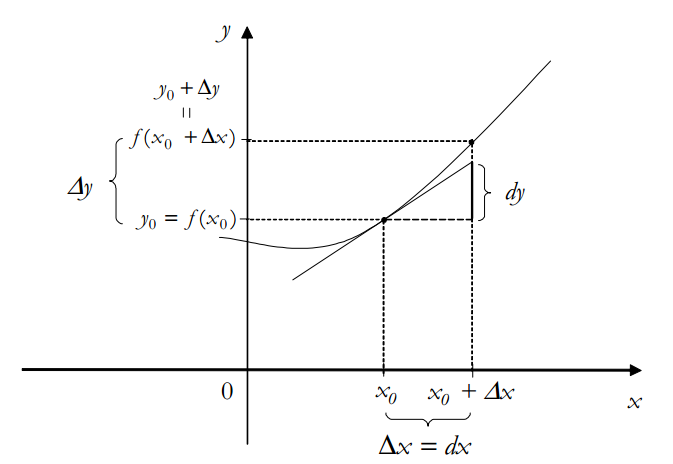
\includegraphics[scale=0.7]{fig_apl_deriv/AplicDerivDiferencial.png}
    \caption{Representação $dy$ e $dx$}
    %\label{fig:my_label}
\end{figure}

Sabemos que $f'(x_0)=\lim_{\Delta x\to 0} \frac{f(x_0+\Delta x)-f(x_0)}{\Delta x}$, o que significa que quando $\Delta x$ está próximo de zero, tem-se $\frac{\Delta y}{\Delta x}$ próximo do coeficiente angular da reta tangente à curva $y= f(x)$ no ponto $(x_0,f(x_0))$, ou seja, $\frac{\Delta y}{\Delta x}\cong f'(x_0)$, se $\Delta x\cong 0$.
A expressão acima pode ser escrita da seguinte forma:
\begin{equation*}
   \Delta y\cong f'(x_0)\Delta x\textrm{, se }\Delta x\cong 0
\end{equation*}
\begin{framed}
\begin{definition}
Sejam $y= f(x)$, onde \f~ é uma função derivável, e $\Delta x$ um acréscimo na variável \x. A diferencial $dy$ da variável dependente $y$ é dada por $dy=f(x)\Delta x$ e a diferencial $dx$ da variável independente \x é dada por $dx=\Delta x$.\\
Em termos gerais, para cálculos aproximados, podemos fazer $f(x+\Delta x)-f(x)=\Delta y \cong dy$, ou seja,
\begin{equation}
    f(x+\Delta x)\cong f(x)+f'(x)\Delta x\label{eq:diferencial}
\end{equation}
\end{definition}
\end{framed}
\begin{ex}
  Vamos determinar aproximadamente o valor de $\sen 31^\circ$. Como não trabalhamos no
Cálculo com a medida angular ``graus'', mas sim com a medida linear ``radianos'', devemos procurar o valor aproximado de $\sen\pc{\frac{\pi}{6}+\frac{\pi}{180}}$. Considerando $f(x)=\sen x$ escrevemos
\begin{equation*}
    \sen(x+\Delta x)\cong\sen x+\cos\Delta x
\end{equation*}
No nosso caso,\\ $\displaystyle\sen\pc{\frac{\pi}{6}+\frac{\pi}{180}}=\sen\frac{\pi}{6}+\cos\frac{\pi}{6\cdot \frac{\pi}{180}}=\frac{1}{2}+\frac{\sqrt{3}}{2}\cdot \frac{\pi}{180}\equiv 0,5+0,8661+0,017=0,5147$
  \end{ex}
  \begin{obs}
    A aplicação da Fórmula \ref{eq:diferencial} já havia sido proposta  \hyperlink{desafio}{neste desafio} do Capítulo \ref{chap:derivadas}. Utilize para calcular uma aproximação para $\sqrt{624}$.
  \end{obs}
  
\section{Teorema do valor médio}\hypertarget{TeoValorMedio}{}\label{sec:TVM}
O Teorema do Valor Médio (TVM) para derivadas é importante na teoria de cálculo por conta das muitas propriedades das funções que podem ser deduzidas a partir dele. Por exemplo, sabemos que funções constantes têm derivadas iguais a zero, mas poderia existir uma função mais complicada cujas derivadas fossem sempre zero? A seguinte teoria nos diz sobre esse assunto.

Para prosseguirmos no entendimento do Teorema do Valor Médio, precisamos primeiro anunciar o Teorema de Rolle. Pois o primeiro é uma aplicação deste.

\subsection{Teorema de Rolle}

O Teorema de Rolle fornece uma condição suficiente para que uma dada função diferenciável tenha derivada nula em pelo menos um ponto.

\begin{framed}
\begin{teo}\normalfont{(Teorema de Rolle)}\label{teo:TeoremaRoole}
  Seja $f$ uma função contínua no intervalo fechado $[a, b]$ e diferenciável no intervalo aberto $(a, b)$. Se
  \begin{equation}
    f(a)=f(b),
  \end{equation}
  então existe pelo menos um {\bf ponto crítico} $c\in (a, b)$ tal que
  \begin{equation}
    f'(c)=0
  \end{equation}
\end{teo}\end{framed}
\begin{figure}[!htb]
  \centering
  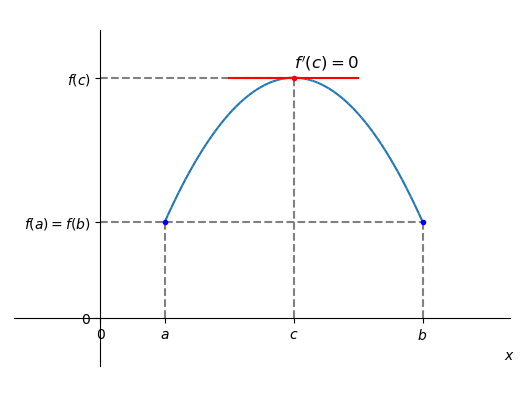
\includegraphics[width=0.6\textwidth]{./fig_apl_deriv/fig_teo_Rolle}
  \caption{Ilustração do Teorema de Rolle.}
  \label{fig:teo_Rolle}
\end{figure}

\nota{ %
No Teorema \ref{teo:TeoremaRoole}:
\begin{compactenum}[a.]
\item a condição de continuidade de \(f\) em \([a,b]\) é obviamente muito importante, pois garante que o gráfico de \(f\) não tenha saltos bruscos dentro de \([a,b]\).
\item afirma-se que a curva deve ter pelo menos uma reta tangente horizontal em algum ponto do intervalo \((a,b)\).
\end{compactenum}
}
\begin{ex}
  O polinômio $p(x) = x^3 - 4x^2 + 3x + 1$ tem pelo menos um ponto crítico no intervalo $(0,1)$ e no intervalo $(1,3)$. De fato,temos $p(0)=p(1)=1$ e, pelo teorema de Rolle, segue que existe pelo menos um ponto $c\in (0, 1)$ tal que $f'(c)=0$. Analogamente, como também $p(1)=p(3)=1$, segue do teorema que existe pelo menos um ponto crítico no intervalo $(1,3)$. Veja o esboço do gráfico de $p$ na Figura \ref{fig:ex_teo_Rolle}.
  \begin{figure}[!htb]
    \centering
    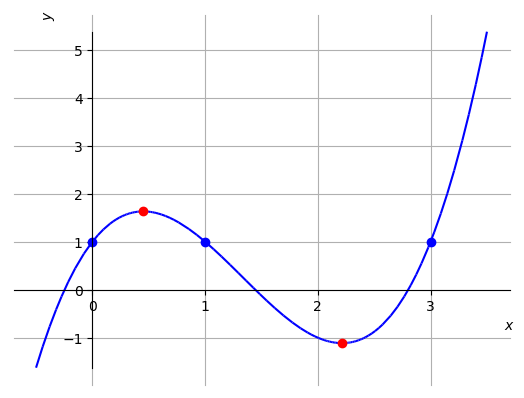
\includegraphics[width=0.6\textwidth]{./fig_apl_deriv/fig_ex_teo_Rolle}
    \caption{Esboço do gráfico de $p(x) = x^3 - 4x^2 + 3x + 1$.}
    \label{fig:ex_teo_Rolle}
  \end{figure}
  
  De fato, como todo polinômio é derivável em toda parte, podemos calcular os pontos críticos como segue.
  \begin{align*}
    p'(x) = 0 &\Rightarrow 3x^2 - 8x + 3 = 0 \\
              &\Rightarrow x = \frac{8 \pm \cancelto{2\sqrt{7}}{\sqrt{64 - 36}}}{6} \\
              &\Rightarrow x_1 = \frac{4 - \sqrt{7}}{3} \cong 0,45 \quad\text{ou}\quad x_2 = \frac{4 + \sqrt{7}}{3} \cong 2,22
  \end{align*}

  
  No \geogebra, podemos usar os seguintes comandos~ para computar os pontos críticos de $p$ e plotar seu gráfico:
\begin{verbatim}
 p(x)= x**3 - 4*x**2 + 3*x + 1
s=soluções (derivada(p))
(s,0)
\end{verbatim}

\end{ex}

\begin{ex}\label{ex:nteo_Rolle}
  Vejamos os seguintes casos em que o Teorema de Rolle não se aplica:
  \begin{enumerate}[a)]
  \item A função
$
      f(x) = \left\{
        \begin{array}{ll}
          x, & 0\leq x < 1\\
          0, & x=1
        \end{array}
      \right.
  $
    é tal que $f(0)=f(1)=0$, entretanto sua derivada $f'(x)=1$ no intervalo $(0, 1)$. Ou seja, a condição da $f$ ser contínua no intervalo fechado associado é necessária no teorema de Rolle. Veja a Figura \ref{fig:ex_fcont_h_2} para o esboço do gráfico desta função.
    
  \begin{figure}[htb]
    \centering
    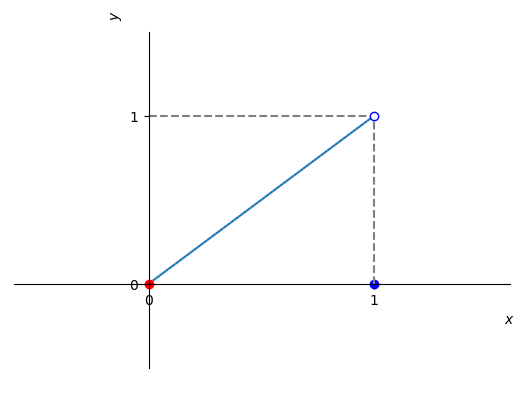
\includegraphics[width=0.6\textwidth]{./fig_apl_deriv/fig_h}
    \caption{Esboço do gráfico da função referente ao Exemplo \ref{ex:nteo_Rolle} a).}
    \label{fig:ex_fcont_h_2}
  \end{figure}
  \item Não existe ponto tal que a derivada da $g(x)=-|x-1|+1$ seja nula. Entretanto, notemos que $g(0)=g(2)=0$ e $g$ contínua no intervalo fechado $[0, 2]$. O teorema de Rolle não se aplica neste caso, pois $g$ não é derivável no intervalo $(0,2)$, mais especificamente, no ponto $x=1$. Veja a Figura \ref{fig:ex_nteo_Rolle_nderiv}.
  \begin{figure}[H]
    \centering
    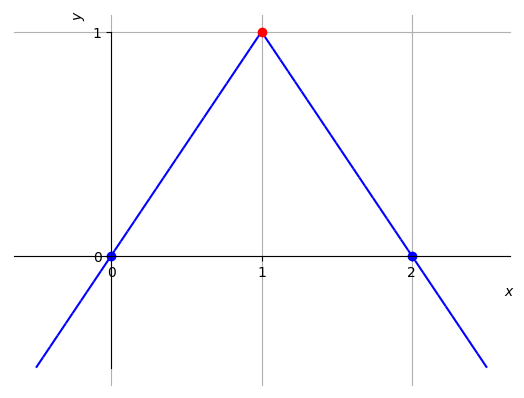
\includegraphics[width=0.5\textwidth]{./fig_apl_deriv/fig_ex_nteo_Rolle_nderiv}
    \caption{Esboço do gráfico da função referente ao Exemplo \ref{ex:nteo_Rolle} b).}
    \label{fig:ex_nteo_Rolle_nderiv}
  \end{figure}  
  \end{enumerate}
\end{ex}

\subsection{Teorema do valor médio }
\begin{framed}
\begin{teo}[Teorema do valor médio ou de Lagrange]~
 \\ Seja $f$ uma função contínua no intervalo fechado $[a,b]$ e diferenciável no intervalo aberto $(a,b)$. Então, existe pelo menos um ponto $c\in (a,b)$ tal que
  \begin{equation}
    \frac{f(b)-f(a)}{b-a}=f'(c)
  \end{equation}
  ou equivalentemente,
\[ f'(c)(b-a)=f(b)-f(a). \]
\end{teo}\end{framed}
\begin{figure}[h]
  \centering
  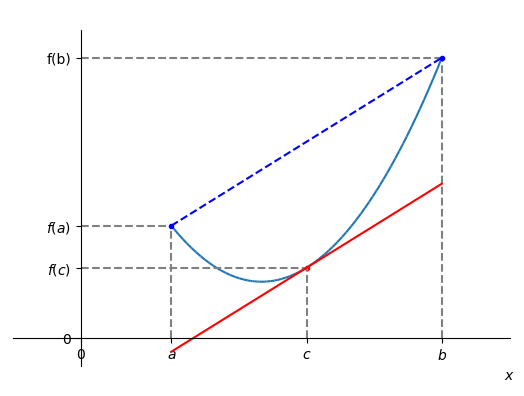
\includegraphics[width=0.55\textwidth]{./fig_apl_deriv/fig_teo_valmed}
  \caption{Ilustração do Teorema do valor médio.}
  \label{fig:teo_valor_medio}
\end{figure}
\begin{obs}
  Em um contexto de aplicação, o Teorema do valor médio relaciona a taxa de variação média da função em um intervalo $[a, b]$ com a taxa de variação instantânea da função em um ponto interior deste intervalo.
\end{obs}

\begin{ex}
  A função $f(x)=x^2$ é contínua no intervalo $[0,2]$ e diferenciável no intervalo $(0,2)$. Logo, segue do teorema do valor médio que existe pelo menos um ponto $c\in (0,2)$ tal que
  \begin{equation}
    f'(c)=\frac{f(2)-f(0)}{2-0}=2
  \end{equation}
  De fato, $f'(x)=2x$ e, portanto, tomando $c=1$, temos $f'(c)=2$.
\end{ex}
\begin{framed}
\begin{corol}[Funções com derivadas nulas são constantes]~
 \\ Se $f'(x)=0$ para todos os pontos em um intervalo $(a, b)$, então $f$ é constante neste intervalo.
\end{corol}
\begin{framed}
\begin{dem}~
\\  De fato, sejam $x_1,x_2\in (a, b)$ e, sem perda de generalidade, $x_1<x_2$. Então, temos $f$ é contínua no intervalo $[x_1,x_2]$ e diferenciável em $(x_1,x_2)$. Segue do teorema do valor médio que existe $c\in (x_1,x_2)$ tal que
  \begin{equation}
    \frac{f(x_2)-f(x_1)}{x_2-x_1}=f'(c)
  \end{equation}
  Como $f'(c)=0$, temos $f(x_2)=f(x_1)$. Ou seja, a função vale sempre o mesmo valor para quaisquer dois ponto no intervalo $(a, b)$, logo é constante neste intervalo.
\end{dem}\end{framed}\end{framed}
\begin{framed}
\begin{corol}[Função com a mesma derivada diferem por uma constante]~\label{corol:apderiv_teomed_2}
 \\ Se $f'(x)=g'(x)$ para todos os pontos em um intervalo aberto $(a,b)$, então $f(x)=g(x)+C$, $C$ constante, para todo $x\in (a,b)$.
\end{corol}
\begin{framed}
\begin{dem}~
   Segue, imediatamente, da aplicação do corolário anterior à função $h(x)=f(x)-g(x)$.
\end{dem}\end{framed}\end{framed}
\begin{framed}
\begin{corol}[Monotonicidade e o sinal da derivada]~\label{corol:mono_deriv}
 \\ Suponha que $f$ seja contínua em $[a,b]$ e derivável em $(a,b)$.
  \begin{itemize}
  \item Se $f'(x)>0$ para todo $x\in (a,b)$, então $f$ é crescente em $[a,b]$.
  \item Se $f'(x)<0$ para todo $x\in (a,b)$, então $f$ é decrescente em $[a,b]$.
  \end{itemize}
\end{corol}
\end{framed}
\begin{ex}
  Vamos estudar a monotonicidade da função polinomial $f(x) = x^3 - 4x^2 + 3x + 1$. Na Figura \ref{fig:ex_corol_mono_deriv}, temos o esboço de seu gráfico.
  
  \begin{figure}[H]
    \centering
    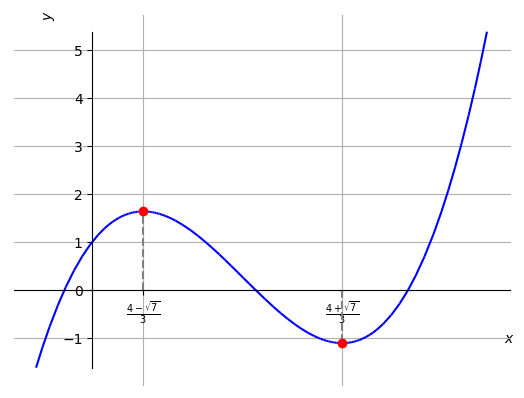
\includegraphics[width=0.55\textwidth]{./fig_apl_deriv/fig_ex_corol_mono_deriv}
    \caption{Esboço do gráfico de $f(x) = x^3 - 4x^2 + 3x + 1$.}
    \label{fig:ex_corol_mono_deriv}
  \end{figure}

  Podemos usar o Corolário \ref{corol:mono_deriv} para estudarmos a monotonicidade (i.e. intervalos de crescimento ou decrescimento). Isto é, fazemos o estudo de sinal da derivada de $f$. Calculamos
  \begin{equation*}
    f'(x) = 3x^2 - 8x + 3
  \end{equation*}
  Logo, temos
  \begin{center}
    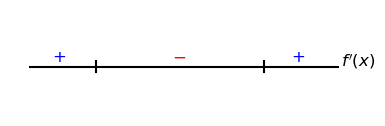
\includegraphics[width=0.5\textwidth]{./fig_apl_deriv/fig_ex_monoderiv_poli}
  \end{center}
  Ou seja, $f'(x) > 0$ no conjunto $\displaystyle \left(-\infty, \frac{4-\sqrt{7}}{3}\right)\cup \left(\frac{4+\sqrt{7}}{3}, \infty\right)$ e $f'(x) < 0$ no conjunto $\displaystyle \left(\frac{4-\sqrt{7}}{3}, \frac{4+\sqrt{7}}{3}\right)$. Concluímos que $f$ é {\bf crescente} nos intervalos $\displaystyle \left(\left.-\infty, \frac{4-\sqrt{7}}{3}\right.\right]$ e $\displaystyle \left[\left.\frac{4+\sqrt{7}}{3}, \infty\right)\right.$, enquanto que $f$ é {\bf decrescente} no intervalo $\displaystyle \left[\frac{4-\sqrt{7}}{3}, \frac{4+\sqrt{7}}{3}\right]$.
\end{ex}

\begin{ex}
  A função exponencial $f(x) = e^x$ é crescente em toda parte. De fato, temos
  \begin{equation*}
    f'(x) = e^x > 0
  \end{equation*}
  para todo $x\in\mathbb{R}$.
\end{ex}

\subsection{Exercícios resolvidos}

\begin{exeresol}
  Um carro percorreu 150 km em 1h30min. Mostre que em algum momento o carro estava a uma velocidade maior que 80 km/h.
\end{exeresol}
\begin{resol}
  Seja $s=s(t)$ a função distância percorrida pelo carro e $t$ o tempo, em horas, contado do início do percurso. Do teorema do valor médio, exite tempo $t_1\in (0,~1,5)$ tal que
  \begin{equation*}
    f'(t_1) = \frac{s(1,5)-s(0)}{1,5-0} = \frac{150}{1,5} = 100~\text{km/h}.
  \end{equation*}
  Ou seja, em algum momento o carro atingiu a velocidade de 100 km/h.
\end{resol}

\begin{exeresol}
  Estude a monotonicidade da função gaussiana $f(x) = e^{-x^2}$.  
\end{exeresol}
\begin{resol}
  Para estudarmos a monotonicidade de uma função, podemos fazer o estudo de sinal de sua derivada. Neste caso, temos
  \begin{equation*}
    f'(x) = -2xe^{-x^2}
  \end{equation*}
  Assim, vemos que
  \begin{center}
    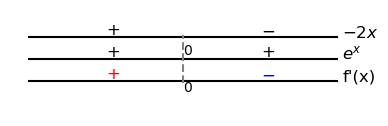
\includegraphics[width=0.5\textwidth]{./fig_apl_deriv/fig_exeresol_gauss_estsinal}
  \end{center}
  Concluímos que $f$ é crescente no intervalo $(-\infty, 0)$ e decrescente no intervalo $(0, \infty)$.
\end{resol}

\subsection{Exercícios}

\begin{exer}
  Estude a monotonicidade de $f(x) = x^2 - 2x$.
\end{exer}
\begin{resp}
  Decrescente: $(-\infty, 1]$; Crescente: $[1, \infty)$
\end{resp}

\begin{exer}
  Estude a monotonicidade de $\displaystyle f(x) = \frac{x^3}{3}-x$.
\end{exer}
\begin{resp}
  Decrescente: $[-1, 1]$; Crescente: $(-\infty, -1]$; $[1, \infty)$
\end{resp}

\begin{exer}
  Estude a monotonicidade de $\displaystyle f(x) = \ln x$.
\end{exer}
\begin{resp}
  Crescente: $(0, \infty)$
\end{resp}


\begin{exer}
  Demonstre que um polinômio cúbico pode ter no máximo $3$ raízes reais.
\end{exer}
\section{Extremos de funções}\label{sec:extremosFunc}
\begin{framed}
\begin{definition}
Seja $f$ uma função com domínio $D$. Dizemos que:
\begin{compactenum}[i.]
\item $f$ tem o valor \emph{máximo global}\footnote{Também chamado de máximo absoluto.} $f(a)$ no ponto $x=a$ quando
\begin{equation}
  f(x) \leq f(a),
\end{equation}
para todo $x\in D$. 
\item  $f$ tem o valor \textbf{mínimo global}\footnote{Também chamado de mínimo absoluto.} $f(b)$ no ponto $x=b$ quando
\begin{equation}
  f(x) \geq f(b),
\end{equation}
para todo $x\in D$. 
\end{compactenum}
Em tais pontos, dizemos que a função têm seus valores \textbf{extremos globais} (ou extremos absolutos).
\end{definition}
\end{framed}

\begin{ex}
 Dada a função \(f(x)=x^3\), determinemos seus valores extremos, caso existam, para os diferentes domínios:
\begin{compactenum}[a.]
\item \({\rm Dom}(f)=\mathbb{R}\)

\begin{solution}
\(f\) não tem valores extremos, pois \(f\) é ilimitada neste domínio. Veja o item (a) da figura abaixo.
\end{solution}
\item \({\rm Dom}(f)=[-2,2]\)

\begin{solution}
\(f\) tem valores extremos em \(-2\) e \(2\), com valor mínimo absoluto \(f(-2)=-8\) e valor máximo absoluto \(f(2)=8\). Veja o item (b) da figura abaixo.
\end{solution}
\begin{figure}[H]
    \centering
    \subfigure[]{\label{fig:intR}%
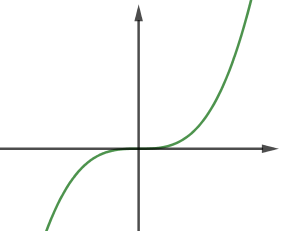
\includegraphics[width=0.25\textwidth]{fig_apl_deriv/IntR}}\hfill
\subfigure[]{\label{fig:[a,b]}%
 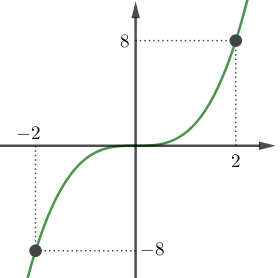
\includegraphics[width=0.22\textwidth]{fig_apl_deriv/Extremos[a,b]}}\hfill
\subfigure[]{\label{fig:(a,b]}%
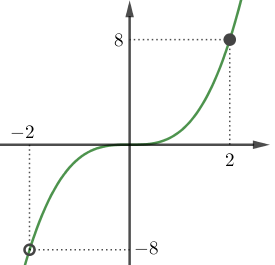
\includegraphics[width=0.22\textwidth]{fig_apl_deriv/Extremos(a,b]}}\hfill
\subfigure[]{\label{fig:(a,b)}%
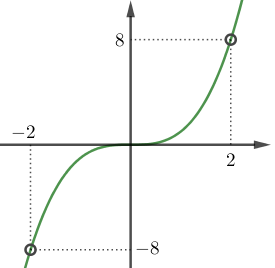
\includegraphics[width=0.22\textwidth]{fig_apl_deriv/Extremos(a,b)}}
\end{figure}
\item \({\rm Dom}(f)=(-2,2]\)

\begin{solution}
\(f\) não tem valores mínimos relativos, pois \(-2 \notin {\rm Dom}(f)\), porém tem um valor extremo em \(2\), com \(f(2)=8\). Veja o item (c) da figura acima.
\end{solution}
\item \({\rm Dom}(f)=(-2,2)\).

\begin{solution}
\(f\) não tem valores extremos, pois \(-2, 2 \notin {\rm Dom}(f)\). Veja o item (d) da figura acima.
\end{solution}
\end{compactenum}
\end{ex}
\begin{ex}\label{ex:vmaxminabs}
  A função $f(x) = x^2$ tem valor mínimo global no ponto $x=0$ e não assume valor máximo global. A função $g(x) = -x^2$ tem valor máximo global no ponto $x=0$ e não assume valor mínimo global. A função $h(x)=x^3$ não assume valores mínimo e máximo globais. Veja a Figura \ref{fig:ex_vmaxminabs}.
  \begin{figure}[!htb]
    \centering
    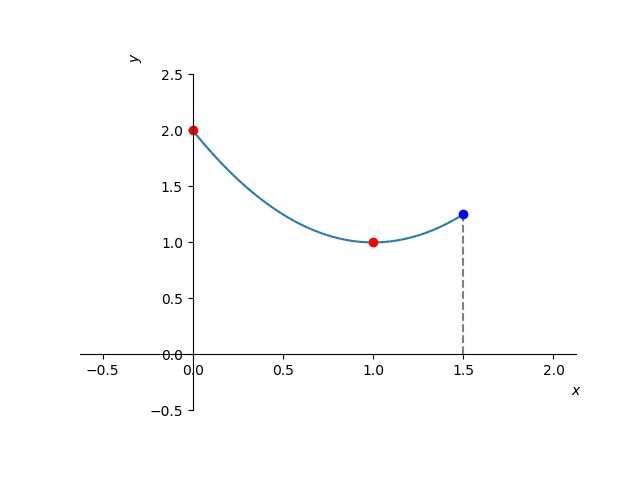
\includegraphics[width=0.35\textwidth]{./fig_apl_deriv/fig_f}~
    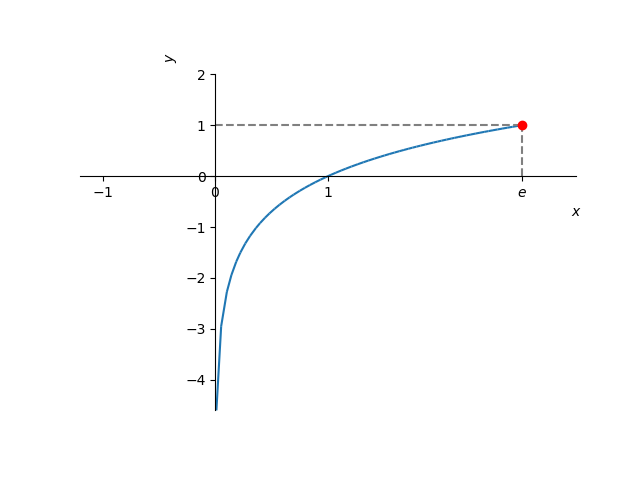
\includegraphics[width=0.35\textwidth]{./fig_apl_deriv/fig_g}~
    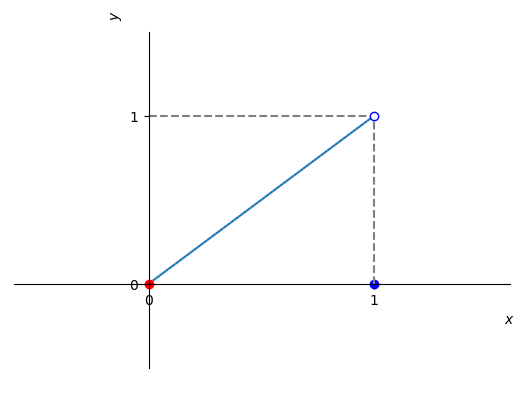
\includegraphics[width=0.35\textwidth]{./fig_apl_deriv/fig_h}
    \caption{Esboço das funções discutidas no Exemplo \ref{ex:vmaxminabs}.}
    \label{fig:ex_vmaxminabs}
  \end{figure}
\end{ex}

\begin{ex}\label{ex:fcont}
  Vejamos os seguintes casos:
  \begin{enumerate}[a)]
  \item  A função $\boldsymbol{f(x) = (x-1)^2+1}$ é contínua no intervalo fechado $\displaystyle \left[0, \frac{3}{2}\right]$. Assume valor mínimo global $1$ no ponto $x=1$. Ainda, assume valor máximo global igual a $2$ no ponto $x=0$. Veja Figura \ref{fig:ex_fcont_f}.
  \begin{figure}[!htb]
    \centering
    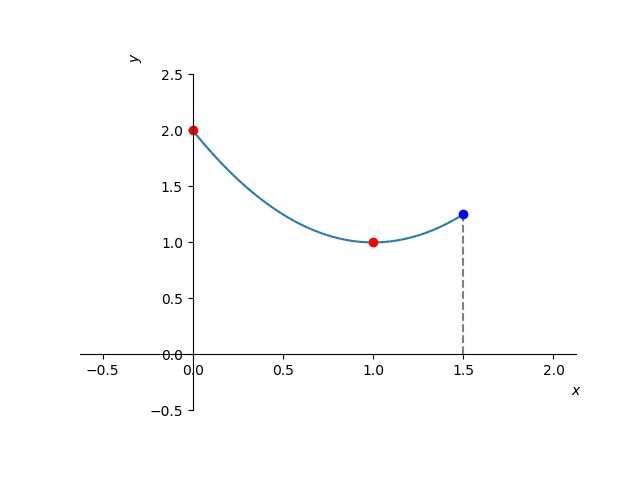
\includegraphics[width=0.6\textwidth]{./fig_apl_deriv/fig_f}
    \caption{Esboço do gráfico de $f(x) = (x-1)^2+1$ no intervalo $\displaystyle\left[0, \frac{3}{2}\right]$. Veja o Exemplo \ref{ex:fcont} a).}
    \label{fig:ex_fcont_f}
  \end{figure}
\item A função $\boldsymbol{g(x) = \ln x}$ é contínua no intervalo $(0, e]$. Neste intervalo, assume valor máximo global no ponto $x=e$, mas não assume valor mínimo global. Veja Figura \ref{fig:ex_fcont_g}.
  \begin{figure}[!htb]
    \centering
    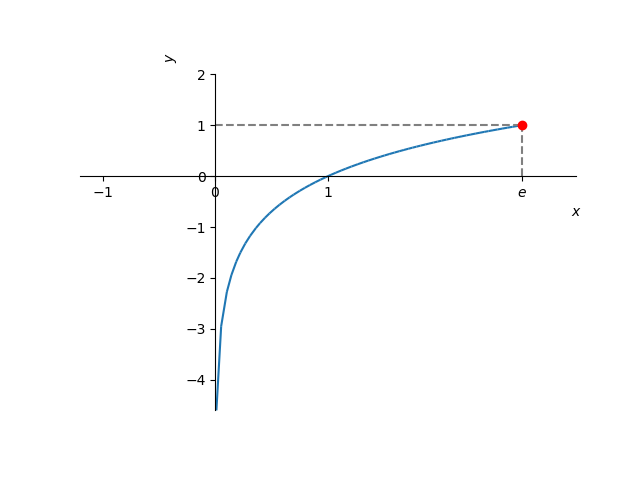
\includegraphics[width=0.6\textwidth]{./fig_apl_deriv/fig_g}
    \caption{Esboço do gráfico de $g(x) = \ln x$ no intervalo $(0,e]$. Veja o Exemplo \ref{ex:fcont} b).}
    \label{fig:ex_fcont_g}
  \end{figure}
  
\item A função
  \begin{equation}
    h(x) = \left\{
      \begin{array}{ll}
        x, & 0\leq x < 1\\
        0, & x=1
      \end{array}
\right.
\end{equation}
definida no intervalo $[0, 1]$ é descontínua no ponto $x=1$. Neste intervalo, assume valor mínimo global no ponto $x=0$, mas não assume valor máximo global. Veja a Figura \ref{fig:ex_fcont_h}.

  \begin{figure}[H]
    \centering
    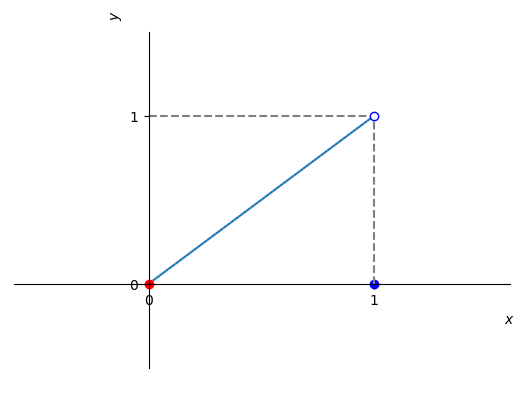
\includegraphics[width=0.6\textwidth]{./fig_apl_deriv/fig_h}
    \caption{Esboço do gráfico de $h(x)$ no intervalo $[0,1]$. Veja o Exemplo \ref{ex:fcont} c).}
    \label{fig:ex_fcont_h}
  \end{figure}
  \end{enumerate}
\end{ex}

\nota{Uma função $f$ tem um valor \emph{máximo local} em um ponto interior $x=a$ de seu domínio, se $f(x) < f(a)$ para todo $x$ em um intervalo aberto em torno de $a$, excluindo-se $x=a$. 

Analogamente, $f$ tem um valor \emph{mínimo local} em um ponto interior $x=b$ de seu domínio, se $f(x) > f(b)$  para todo $x$ em um intervalo aberto em torno de $b$, excluindo-se $x=b$. 

Em tais pontos, dizemos que a função têm valores \emph{extremos locais} (ou relativos). Um tal ponto é chamado de \emph{ponto de máximo local} ou \emph{de mínimo local}, conforme o caso.}
 \begin{ex}\label{ex:vmaxminloc}
  Consideremos a função
  \begin{equation*}
    f(x) = \left\{
      \begin{array}{ll}
        -(x+1)^2-2, & -2\leq x < -\frac{1}{2},\\
        |x|, & -\frac{1}{2} \leq x < 1,\\
        (x-2)^3+2, & 1\leq x < 3.
      \end{array}
\right.
\end{equation*}

Na Figura \ref{fig:ex_vmaxminloc} temos o esboço de seu gráfico. Por inferência, temos que $f$ tem valores máximos locais nos pontos $x=-1$ e $x=-1/2$. No ponto $x=0$ tem um valor mínimo local. Observamos que $x=-2$, $x=2$ e $x=3$ não são pontos de extremos locais desta função. No ponto $x=-2$, $f$ tem seu valor mínimo global. Ainda, $f$ não tem valor máximo global.
\end{ex}
 \begin{figure}[hbt]
    \centering
    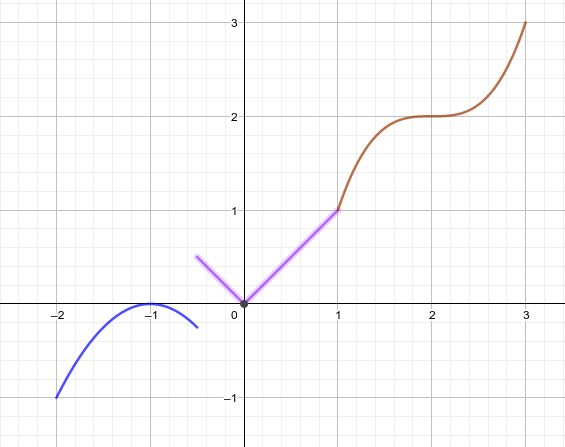
\includegraphics[width=0.6\textwidth]{fig_apl_deriv/FuncPartValMaxMin}
    \caption{Esboço do gráfico de $f(x)$ discutida no Exemplo \ref{ex:vmaxminloc}.}
    \label{fig:ex_vmaxminloc}
  \end{figure}
  
  \begin{framed}
\begin{teo}[\normalfont{Teorema do valor extremo}]~\label{teo:ValorExt}
Se \(f\) é uma função contínua em um intervalo fechado e limitado \([a,b]\), então \(f\) atinge tanto um valor máximo absoluto \(M\) quanto um valor mínimo absoluto \(m\) neste intervalo. Isto é, existem \(x_1,\,\,\,x_2\in[a,b]\) tais que:
\[ f(x_1)=m,\quad f(x_2)=M\quad \mbox{e}\quad m\leq f(x)\leq M\quad \mbox{para qualquer} \quad x \in [a,b]. \]
\end{teo}\end{framed}

A seguinte Nota ilustra algumas possíveis localizações dos valores extremos de uma função contínua em um intervalo fechado \([a,b]\)
\begin{figure}[H]
    \centering
    \subfigure[]{\label{fig:TVext1}%
\includegraphics[width=0.25\textwidth]{fig_apl_deriv/TVext1}}\hfill
\subfigure[]{\label{fig:TVext2}%
 \includegraphics[width=0.22\textwidth]{fig_apl_deriv/TVext2}}\hfill
\subfigure[]{\label{fig:TVext33}%
\includegraphics[width=0.22\textwidth]{fig_apl_deriv/TVext33}}\hfill
\subfigure[]{\label{fig:TVext4}%
\includegraphics[width=0.22\textwidth]{fig_apl_deriv/TVext4}}
\end{figure}

\nota{%
\hspace{-1cm}\begin{itemize}
\item No item (a), \(f\) tem valores extremos em \(x_2\) e \(x_1\), e estão no interior de \([a,b]\);
\item No item (b), \(f\) tem valores extremos nas extremidades do intervalo \(a\) e \(b\);
\item No item (c), \(f\) tem valores extremos em \(x_3\), ponto interior de \([a,b]\), e na extremidade \(a\);
\item No item (d), \(f\) tem valores extremos em \(x_4\), ponto interior de \([a,b]\), e na extremidade \(b\).
\end{itemize}
}

No Teorema \ref{teo:ValorExt}, as hipóteses do intervalo ser fechado e limitado, e a função ser contínua, são hipóteses fundamentais, sem estas, as conclusões não são válidas. Por exemplo, a função \(f(x)=\ln(x)\) é contínua no intervalo aberto \((0,1)\), porém, não tem valores extremos.

  
\begin{framed}
\begin{teo}[\normalfont{Teorema da derivada para pontos extremos locais}]~
\\  Se $f$ possui um valor extremo local em um ponto $x=a$ e $f$ é diferenciável neste ponto, então
  \begin{equation*}
    f'(a) = 0
  \end{equation*}
\end{teo}\end{framed}

Deste teorema, podemos concluir que uma função $f$ pode ter valores extremos em:
\begin{enumerate}
\item pontos interiores de seu domínio onde $f' = 0$,
\item pontos interiores de seu domínio onde $f'$ não existe, ou
\item pontos extremos de seu domínio.
\end{enumerate}

Um ponto interior do domínio de uma função $f$ onde $f'=0$ ou $f'$ não existe, é chamado de \emph{ponto crítico} da função.

\begin{obs}\label{obs:pt_critico_val_extremo}
  Uma função tem valores extremos em pontos críticos ou nos extremos de seu domínio.
\end{obs}


\begin{ex}
  Consideramos a função $f(x)$ discutida no Exemplo \ref{ex:vmaxminloc}. No ponto $x=-1$, $f'(-1)=0$ e $f$ tem valor máximo local neste ponto. Entretanto, no ponto $x=2$, também temos $f'(2)=0$, mas $f$ não tem valor extremo neste ponto.

  No ponto $x=0$, $f'(0)$ não existe e $f$ tem valor mínimo local neste ponto. No ponto, $x=-1/2$, $f'(1/2)$ não existe e $f$ tem valor máximo local neste ponto.

  Nos extremos do domínio, temos que $f$ tem valor mínimo global no ponto $x=-2$, mas não tem extremo global no ponto $x=3$.
\end{ex}

\subsection{Exercícios resolvidos}

\begin{exeresol}\label{exeresol:f_diff}
  Determine os pontos extremos da função $f(x) = (x+1)^2-1$ no intervalo $[-2,1]$.
\end{exeresol}
\begin{resol}
  Os valores extremos de um função podem ocorrer, somente, em seus pontos críticos ou nos extremos de seu domínio. Como $f(x) = (x+1)^2-1$ é diferenciável no intervalo $(-2,1)$, seus pontos críticos são pontos tais que $f'=0$. Para identificá-los, calculamos
  \begin{align*}
    f'(x)=0 &\Rightarrow 2(x+1) = 0\\
            &\Rightarrow x = -1
  \end{align*}

  \begin{figure}[htb]
    \centering
    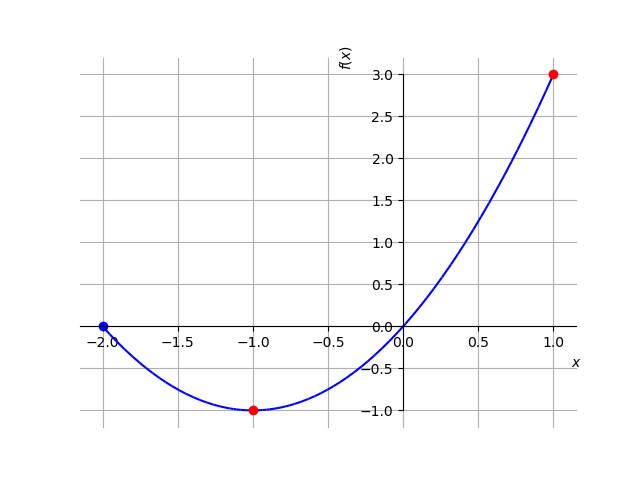
\includegraphics[width=0.7\textwidth]{./fig_apl_deriv/fig_exeresol_f_diff}
    \caption{Esboço do gráfico da função $f(x) = (x+1)^2-1$ discutida no Exercício Resolvido \ref{exeresol:f_diff}.}
    \label{fig:exeresol_f_diff}
  \end{figure}

  Desta forma, $f$ pode ter valores extremos nos ponto $x=-2$, $x=-1$ e $x=1$. Analisamos, então, o esboço do gráfico da função (Figura \ref{fig:exeresol_f_diff}) e a seguinte tabela:\\
  \begin{center}
  \begin{tabular}[H]{l|ccc}
    $x$ & -2 & -1 & 1 \\\hline
    $f(x)$ & 0 & -1 & 3\\\hline
  \end{tabular}
\end{center}
Daí, podemos concluir que $f$ tem o valor mínimo global (e local) de $f(-1)=-1$ no ponto $x=-1$ e tem valor máximo global de $f(1)=3$ no ponto $x=1$.


Podemos usar o \geogebra~para computar os pontos extremos e plotar a função. Por exemplo, com os seguintes comandos~:
\begin{verbatim}
 f(x)= (x+1)**2-1
solucoes(derivada(f))
f(-2)
f(-1)
f(1)
\end{verbatim}
\end{resol}
\begin{exeresol}\label{exeresol:p_infl}
  Determine os pontos extremos da função $f(x)=x^3$ no intervalo $[-1, 1]$.
\end{exeresol}
\begin{resol}
  Como $f$ é diferenciável no intervalo $(-1, 1)$, temos que seus pontos críticos são tais que $f'(x)=0$. Neste caso, temos
  \begin{equation}
    3x^2=0\Rightarrow x=0
  \end{equation}
  é o único ponto crítico de $f$. Entretanto, analisando o gráfico desta função (Figura \ref{fig:exeresol_p_infl}) vemos que $f$ não tem valor extremo local neste ponto. Assim, seus pontos extremos só podem ocorrer nos extremos do domínio $[-1, 1]$. Concluímos que $f(-1)=-1$ é o valor mínimo global de $f$ e $f(1)=1$ é seu valor máximo global.

  \begin{figure}[H]
    \centering
    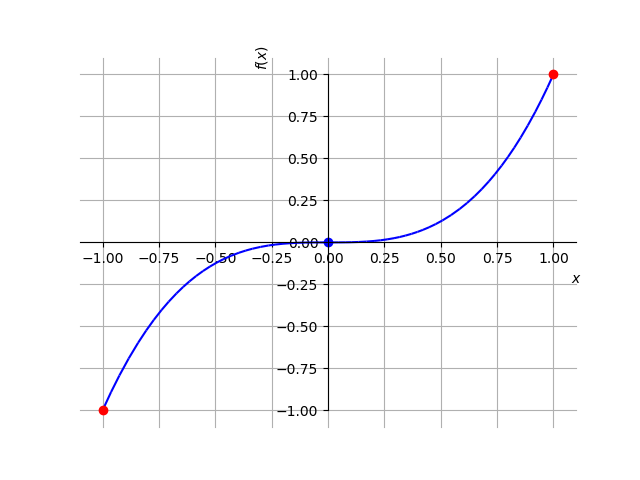
\includegraphics[width=0.7\textwidth]{./fig_apl_deriv/fig_exeresol_p_infl}
    \caption{Esboço do gráfico da função $f(x) = x^3$ discutida no Exercício Resolvido \ref{exeresol:p_infl}.}
    \label{fig:exeresol_p_infl}
  \end{figure}
\end{resol}

\subsection{Exercícios}

\begin{exer}
  Considere que uma dada função $f$ tenha o seguinte esboço de gráfico:

  \begin{center}
    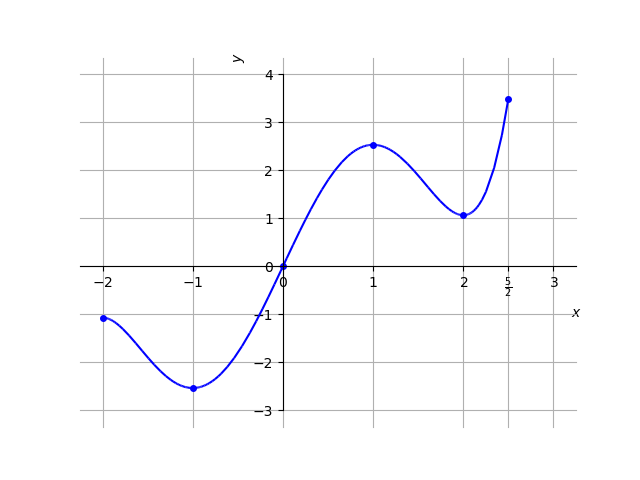
\includegraphics[width=0.7\textwidth]{./fig_apl_deriv/fig_exer_extfun}
  \end{center}

  Determine e classifique os pontos extremos desta função.
\end{exer}
\begin{resp}
  $x=-1$ ponto de mínimo global; $x=1$ ponto de máximo local; $x=2$ ponto de mínimo local; $x=\frac{5}{2}$ ponto de máximo global.
\end{resp}

\begin{exer}
  Dada a função $f(x)=x^2-2x+3$ restrita ao intervalo $[-1,2]$, determine:
  \begin{enumerate}[a)]
  \item seu(s) ponto(s) crítico(s).
  \item seu(s) ponto(s) extremo(s) e o(s) classifique.
  \item seu(s) valor(es) extremo(s) e o(s) classifique.
  \end{enumerate}
\end{exer}
\begin{resp}
  a)~$x=1$; b)~$x=-1$ ponto de máximo global; $x=1$ ponto de mínimo local e global; c)~$f(-1)=6$ valor máximo global; $f(1)=2$ valor mínimo local e global;
\end{resp}

\begin{exer}
  Dada a função $f(x)=-x^2+2x+1$ restrita ao intervalo $[0,3]$, determine:
  \begin{enumerate}[a)]
  \item seu(s) ponto(s) crítico(s).
  \item seu(s) ponto(s) extremo(s) e o(s) classifique.
  \item seu(s) valor(es) extremo(s) e o(s) classifique.
  \end{enumerate}
\end{exer}
\begin{resp}
  a)~$x=1$; b)~$x=1$ ponto de máximo local e global; $x=3$ ponto de mínimo global; c)~$f(1)=2$ valor máximo local e global; $f(3)=-2$ valor mínimo global;
\end{resp}

\begin{exer}
  Dada a função $f(x)=x^{3} - 3 x^{2} + 3 x$ restrita ao intervalo $[0, \infty)$, determine:
  \begin{enumerate}[a)]
  \item seu(s) ponto(s) crítico(s).
  \item seu(s) ponto(s) extremo(s) e o(s) classifique.
  \item seu(s) valor(es) extremo(s) e o(s) classifique.
  \end{enumerate}
\end{exer}
\begin{resp}
  a)~$x=1$; b)~$x=0$ ponto de mínimo global;c)~$f(0)=0$ valor mínimo global;
\end{resp}

\begin{exer}
  Dada a função $f(x)=x^{1/3}$ restrita ao intervalo $[-1,1]$, determine:
  \begin{enumerate}[a)]
  \item seu(s) ponto(s) crítico(s).
  \item seu(s) ponto(s) extremo(s) e o(s) classifique.
  \item seu(s) valor(es) extremo(s) e o(s) classifique.
  \end{enumerate}
\end{exer}
\begin{resp}
  a)~$x=0$; b)~$x=-1$ ponto de mínimo global; $x=1$ ponto de máximo global; c)~$f(-1)=-1$ valor mínimo global; $f(1)=1$ valor máximo global;
\end{resp}
\section{Crescimento e Decrescimento de funções}\hypertarget{Func-CrescDecresc}{}\label{sec:FuncCrescDecresc}
\begin{framed}
\begin{definition}~
\begin{compactenum}[i.]
\item Uma função $f$ é crescente (ou está estritamente aumentando) em um intervalo $I$ se para cada $x_1, x_2 \in I$ com $x_1 <x_2$, $f (x_1) <f (x_2)$ [ou seja, $f (x) $aumenta à medida que $x$ aumenta].\\
\item Uma função \(f\) é decrescente (ou está estritamente) diminuindo) no intervalo $I$ se para cada $x_1, x_2 \in I$
com $x_1 <x_2$, $f (x_1) >f (x_2)$ [ou seja, $f (x) $ fica menor à medida que $x$ fica maior].
\end{compactenum}
\end{definition}
\end{framed}

Por que nos preocupamos com uma definição tão óbvia? Claro, qualquer um pode olhar para um
gráfico de uma função e veja imediatamente onde essa função está aumentando e diminuindo. O verdadeiro desafio é determinar onde uma função está aumentando e diminuindo, dada apenas uma fórmula matemática para a função. Por exemplo, você pode determinar onde $f (x) = x^2 \sin x$ está aumentando e diminuindo, sem olhar para um gráfico? Olhe atentamente na Figura \ref{Fig:FuncCrescDecresc}    para ver se você pode perceber o que acontece em todos os pontos em que a função está aumentando ou diminuindo. 
\begin{figure}[!htb]
    \centering
    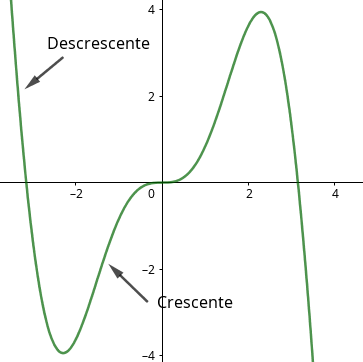
\includegraphics[scale=0.6]{fig_apl_deriv/Cresc_Decresc.png}
    \caption{Crescimento e decrescimento da função $f(x)=x^2\sin (x)$}
    \label{Fig:FuncCrescDecresc}
\end{figure}

O próximo teorema, anunciado a seguir, nos fornecerá elementos para classificar os intervalos em que uma função é crescente ou decrescente manipulando apenas a expressão da mesma.
\begin{teo}
Suponha que $f$ seja diferenciável em um intervalo $I$.
\begin{compactenum}[(i)]
\item se  $f'(x)> 0$ para todo $ x\in I$, então $f$ é crescente em $I$.
\item  se $f'(x) <0$ para todo $ x\in I$, então $f$ é decrescente em $I$.
\end{compactenum}
\end{teo}

\begin{ex}
 Vamos verificar os intervalos em que a função $f ( x ) = 2 x^3 + 9 x^2 - 24x - 10$ é crescente ou decrescente.\\
 \begin{solution}
Observe que $f'(x)=6x^2+18x-24=6(x-1)(x+4)$. Os pontos críticos de $f'$ ocorrem para os valores  $x=1$ e $x=-4 $. Desta forma, devermos avaliar o sinal de $f'$ em relação a estes valores de $x$.
\begin{itemize}
    \item Para $x<-4$, temos que  $(x-1)<0$ e $(x+4)<0$ e consequentemente $f'(x)=6(x-1)(x+4)>0$. Então $f$ é crescente.
    \item para $-4<x<1$ temos que $(x-1)<0$ e $(x+4)>0$ e consequentemente $f'(x)=6(x-1)(x+4)<0$. Então $f$ é decrescente.
    \item para $x>1$ temos que $(x-1)>0$ e $(x+4)>0$ e consequentemente $f'(x)=6(x-1)(x+4)>0$. Então $f$ é crescente.
\end{itemize}
Com isso, temos
  \begin{center}
  \begin{tabular}{lccc}\hline
    Intervalo & $x<-4$ & $-4<x<1$ & $x>1$ \\\hline
    $f'$ & + & - & + \\
    $f$ & crescente & decrescente & crescente\\\hline
  \end{tabular}
\end{center}
Conclusão: A função $f$ é crescente no intervalo $(-\infty,-4)\cup (1,\infty)$ e decrescente no intervalo $(-4,1)$.
 \end{solution}
\end{ex}

\section{Máximos e Mínimos de funções}\hypertarget{MaxMin}{}\label{sec:MaxMin}
Na Seção \ref{sec:extremosFunc}, vimos que os extremos de uma função ocorrem nos extremos de seu domínio ou em um ponto crítico. Aliado a isso, o Corolário \ref{corol:mono_deriv} nos fornece condições suficientes para classificar os pontos críticos como extremos locais.

Mais precisamente, seja $c$ um ponto crítico de uma função contínua $f$ e diferenciável em todos os pontos de um intervalo aberto $(a, b)$ contendo $c$, exceto possivelmente no ponto $c$. Movendo-se no sentido positivo em $x$:
\begin{itemize}
\item se $f'(x)$ muda de negativa para positiva em $c$, então $f$ possui um mínimo local em $c$;
\item se $f'(x)$ muda de positiva para negativa em $c$, então $f$ possui um máximo local em $c$;
\item se $f'$ não muda de sinal em $c$, então $c$ não é um extremo local de $f$.
\end{itemize}
Veja a Figura \ref{fig:tder1}.

\begin{figure}[H]
  \centering
  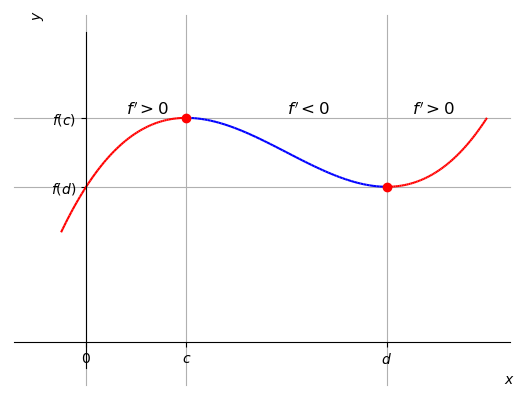
\includegraphics[width=0.6\textwidth]{./fig_apl_deriv/fig_tder1}
  \caption{Ilustração do teste da primeira derivada com $c$ ponto de máximo local e $d$ ponto de mínimo local.}
  \label{fig:tder1}
\end{figure}
\subsection{Teste da primeira derivada}
O teorema abaixo formaliza o explicitado.
\begin{framed}
\begin{teo}[Teste da primeira derivada]~
\\ Seja $f$ uma função contínua no intervalo $[a, b]$ e derivável em  $(a,b)$, exceto possivelmente em $x=c\in (a,b)$.
\begin{compactenum}[(a)]
\item Se $f'(x)>0$, para $a<x<c$ e $f'(x)<0$ para $c<x<b$, então $f$ tem um máximo local em $x=c$.
\item  Se $f'(x)<0$, para $a<x<c$ e $f'(x)>0$ para $c<x<b$, então $f$ tem um mínimo local em $x=c$.
\end{compactenum}
\end{teo}
\end{framed}
\begin{ex}
  Consideremos a função $\displaystyle f(x)=\frac{x^3}{3}-2x^2+3x+3$. Como $f$ é diferenciável em toda parte, seus pontos críticos são aqueles tais que
  \begin{equation}
    f'(x)=0
  \end{equation}
  Temos $f'(x) = x^2 - 4x + 3$. Segue, que os pontos críticos são
  \begin{align*}
    x^2-4x+3=0 &\Rightarrow x = \frac{4\pm \cancelto{2}{\sqrt{16-12}}}{2} \\
    &\Rightarrow x_1 = 1,\quad x_2=3.
  \end{align*}
  Com isso, temos
  \begin{center}
  \begin{tabular}{lccc}\hline
    Intervalo & $x<1$ & $1<x<3$ & $3<x$ \\\hline
    $f'$ & + & - & + \\
    $f$ & crescente & decrescente & crescente\\\hline
  \end{tabular}
\end{center}
  Então, do teste da primeira derivada, concluímos que $x_1=1$ é ponto de máximo local e que $x_2=3$ é ponto de mínimo local.\\
 \begin{quote}
Podemos usar o \geogebra~ para computarmos a derivada de $f$ com o comando:\\
\verb|f(x)=derivada(x**3/3-2*x**2+3*x+3)|\\
  Então, podemos resolver $f'(x)=0$ com o comando\\
\verb+s=soluções(f)+\\
  e, por fim, podemos fazer o estudo de sinal da $f'$ utilizando \verb=f<0= e \verb=f>0= separadamente.
  \end{quote}
\end{ex}

\begin{ex}
 Determinemos os intervalos de crescimento e decrescimento, e os valores extremos de \(f\):
 \begin{compactenum}[a)]
 \item \(f(x)=2x^3+6x^2-48x+9\)
 
 \begin{solution}
 \begin{compactenum}[1.]
 \item \({\rm Dom}(f)=\mathbb{R}\);
\item Da definição de \(f\), temos que \(f'(x)=6x^2+12x-48=6(x+4)(x-2)\).
Logo, os pontos críticos são:
\[ x=-4\quad \mbox{e}\quad x=2. \]
e os intervalos onde analisaremos se \(f\) é crescente ou decrescente são:
\[ (-\infty,-4),\quad(-4,2)\quad \mbox{e}\quad (2,+\infty). \]
\begin{center}
  \begin{tabular}{l|c|c}
  \toprule
    \textbf{Intervalos} &	\emph{Sinal de \(f'\)} &	\textbf{Cresc. ou Decresc.}\\\hline
\((-\infty,-4)\) &\(+\)& cresce\\\hline
\((-4,2)\)&\(-\)&decresce\\\hline
\((2,+\infty)\)&\(+\)& cresce\\
\bottomrule
  \end{tabular}
  \end{center}
   \end{compactenum}
 Portanto, do critério da derivada primeira para encontrar valores extremos, temos que:
\begin{itemize}
    \item \(f(-4)=169\) é um valor máximo relativo (ou local), em \(x=-4\);
\item \(f(2)=-47\) é um valor mínimo relativo (ou local), em \(x=2\).
\end{itemize}
 \end{solution}
 \item \(f(x)=\dfrac{4}{x-1}+\dfrac{3x+2}{3}\)
 
 \begin{solution}
 \begin{compactenum}[1.]
 \item \({\rm Dom}(f)=\mathbb{R}\setminus\{1\}\);
\item Da definição de \(f\), temos que \(f'(x)=-\dfrac{4}{(x-1)^2}+ \dfrac{3}{3}=\dfrac{(x+1)(x-3)}{(x-1)^2}\).
Note que, \(x=1\) não é um ponto crítico, pois \(1\notin {\rm Dom}(f)\). Logo, os pontos críticos são:

\[ x=-1\quad\mbox{e}\quad x=3. \]
e os intervalos onde analisaremos se \(f\) é crescente ou decrescente são:

\[ (-\infty,-1),\quad(-1,1),\quad (1,3)\quad \mbox{e}\quad (3,+\infty). \]
\begin{center}
  \begin{tabular}{l|c|c}
  \toprule
    \textbf{Intervalos} &	\emph{Sinal de \(f'\)} &	\textbf{Cresc. ou Decresc.}\\\hline
\((-\infty,-1)\) &\(+\)& cresce\\\hline
\((-1,1)\)&\(-\)&decresce\\\hline
\((1,3)\) & \(-\) & decresce\\\hline
\((3,+\infty)\)&\(+\)& cresce\\
\bottomrule
  \end{tabular}
  \end{center}
   \end{compactenum}
 Portanto, do critério da derivada primeira para encontrar valores extremos, temos que:
\begin{itemize}
    \item \(f(-1)=- \dfrac{7}{3} \) é um mínimo relativo;
\item \(f(3)= \dfrac{17}{3} \) é um máximo relativo.
\end{itemize}
 \end{solution}
 \item \(f(x)=3x^{1/3}(x+4)^{2/3}\)
 
 \begin{solution}
 \begin{compactenum}[1.]
 \item \({\rm Dom}(f)=\mathbb{R}\);
\item Da definição de \(f\), temos que \(f'(x)=\dfrac{(x+4)^{2/3}}{x^{2/3}}+ \dfrac{2x^{1/3}}{(x+4)^{1/3}}=\dfrac{3x+4}{x^{2/3}(x+4)^{1/3}}\).
Logo, os pontos críticos são:

\[ x=-4,\quad x=-\dfrac{4}{3}\quad\mbox{e}\quad x=0. \]
e os intervalos onde analisaremos se \(f\) é crescente ou decrescente são:

\[ (-\infty,-4),\quad\left(-4,-\dfrac{4}{3}\right),\quad \left(-\dfrac{4}{3},0\right)\quad \mbox{e}\quad (0,+\infty). \]
\begin{center}
  \begin{tabular}{l|c|c}
  \toprule
    \textbf{Intervalos} &	\emph{Sinal de \(f'\)} &	\textbf{Cresc. ou Decresc.}\\\hline
\((-\infty,-4)\) &\(+\)& cresce\\\hline
\(\left(-4,-\frac{4}{3}\right)\)&\(-\)&decresce\\\hline
\(\left(-\frac{4}{3},0\right)\) & \(+\) & cresce\\\hline
\((0,+\infty)\)&\(+\)& cresce\\
\bottomrule
  \end{tabular}
  \end{center}
   \end{compactenum}
Portanto, do critério da derivada primeira para encontrar valores extremos, temos que:
\begin{itemize}
    \item \(f(-4)=0 \) é um máximo relativo;
\item \(f\left(-\dfrac{4}{3}\right)=-4\sqrt[3]{4}\) é um mínimo relativo;
\item \(f(0)=0\), porém não é extremo relativo.
\end{itemize}
 \end{solution}
 \item \(f(x)=\left\{\begin{array}{ll} \sqrt{16-(x+3)^2},& \mbox{se }-7\leq x\leq 1;\\ 1-x^2,& \mbox{se }x> 1\\ \end{array}\right.\)
 
 \begin{solution}
 \begin{compactenum}[1.]
 \item \({\rm Dom}(f)=[-7,+\infty)\);
\item Da definição de \(f\), temos que \(f'(x)=\left\{\begin{array}{ll} -\dfrac{x+3}{\sqrt{16-(x+3)^2}},& \mbox{se }-7<x< 1\\ -2x,& \mbox{se }x> 1\\ \end{array}\right.\).
Note que,
\begin{itemize}
    \item \(x=0\) não é um ponto crítico, pois \(f'(x)=-2x\) está definida para todo \(x>1\), e \(0<1\);
    \item \(x=-7\) não é um ponto crítico, pois não pertence ao interior de \({\rm Dom}(f)\).
    \end{itemize}
    Logo, os pontos críticos são:

\[ x=-3 \quad \mbox{e}\quad x=1. \]
e os intervalos onde analisaremos se \(f\) é crescente ou decrescente são:

\[ (-7,-3),\quad(-3,1)\quad \mbox{e}\quad (1,+\infty). \]

\begin{center}
  \begin{tabular}{l|c|c}
  \toprule
    \textbf{Intervalos} &	\emph{Sinal de \(f'\)} &	\textbf{Cresc. ou Decresc.}\\\hline
    \((-7,-3)\) &\(+\)& cresce\\\hline
    \((-3,1)\)&\(-\)&decresce\\\hline
    \((1,+\infty)\) & \(+\) & decresce\\
    \bottomrule
  \end{tabular}
  \end{center}
\end{compactenum}
Portanto, do critério da derivada primeira para encontrar valores extremos, temos que:
\begin{itemize}
    \item \(f(-3)=4 \) é um máximo relativo;
    \item \(f(0)=0\) não é extremo relativo.
\end{itemize}
 \end{solution}
 \end{compactenum}
\end{ex}

\subsection{Exercícios resolvidos}
%\addcontentsline{toc}{subsection}{Exercícios resolvidos}
\begin{exeresol}
  Determine e classifique os extremos da função
  \begin{equation*}
    f(x) = x^4 - 4x^3 + 4x^2
  \end{equation*}
\end{exeresol}
\begin{resol}
  Como o domínio da $f$ é $(-\infty, \infty)$ e $f$ é diferenciável em toda parte, temos que seus extremos ocorrem em pontos críticos tais que
  \begin{equation*}
    f'(x)=0
  \end{equation*}
  Resolvendo, obtemos
  \begin{align*}
    4x^3-12x^2+8x=0 &\Rightarrow 4x(x^2-3x+2)=0
  \end{align*}
  Logo,
  \begin{align*}
    4x=0 \quad\text{ou}\quad &x^2-3x+2=0\\
    x_1 = 0  \quad\text{ou}\quad     &x = \frac{3\pm 1}{2} \\
                             &x_2 = 1,\quad x_3=2
  \end{align*}
  Portanto, os ponto críticos são $x_1=0$, $x_2=1$ e $x_3=2$. Fazendo o estudo de sinal da $f'$, temos
  \begin{center}
    \begin{tabular}{lcccc}\hline
                 & $x<0$ & $0<x<1$ & $1<x<2$ & $2<x$ \\\hline
      $4x$       & -       &     +       &     +      &   +  \\
      $x^2-3x+2$ & +       &     +       &     -      &   +   \\
      $f'(x)$    & -       &     +       &     -      &   +   \\
      $f$        & decrescente & crescente & decrescente & crescente \\\hline
    \end{tabular}\\
  \end{center}
  Então, do teste da primeira derivada, concluímos que $x_1=0$ é ponto de mínimo local, $x_2=-2$ é ponto de máximo local e $x_3=-1$ é ponto de mínimo local.

  
  Podemos usar os seguintes comandos do \geogebra~ para resolvermos este exercício de maneira análoga ao anterior.
\end{resol}

\begin{exeresol}
  Encontre o valor máximo global de $f(x) = (x-1)e^{-x}$.
\end{exeresol}
\begin{resol}
  Como $f$ é diferenciável em toda parte, temos que seu máximo ocorre em ponto crítico tal que
  \begin{align*}
    f'(x) = 0 &\Rightarrow (2-x)e^{-x} = 0 \\
              &\Rightarrow 2-x = 0 \\
              &\Rightarrow x = 2
  \end{align*}
  Fazendo o estudo de sinal da derivada, obtemos
  \begin{center}
    \begin{tabular}[H]{lcc}
         & x<0 & 0<x \\\hline
      f' & + & - \\
      f  & crescente & decrescente \\\hline
    \end{tabular}
  \end{center}
  Portanto, do teste da primeira derivada, podemos concluir que $x=2$ é ponto de máximo local. O favor da função neste ponto é $f(2) = e^{-2}$. Ainda, temos
  \begin{align*}
    &\lim_{x\to -\infty} (x-1)e^{-x} = -\infty, \\
    &\lim_{x\to \infty} (x-1)e^{-x} = 0
  \end{align*}
  Por tudo isso, concluímos que o valor máximo global de $f$ é $f(2) = e^{-2}$.

  Podemos usar os seguintes comandos do \geogebra~ para resolvermos este exercício:
\begin{verbatim}
f(x)=(x-1)e^(-x)
g(x)= f'(x)
s=soluções(g)
 g'(x) < 0
g'(x) > 0
 limite f(x),-oo)
 limite f(x),oo)
 f(2)
\end{verbatim}
\end{resol}
\subsection{Exercícios}
\begin{exer}
  Use o teste da primeira derivada para encontrar e classificar o(s) ponto(s) extremo(s) de $f(x) = x^2 - 2x$.
\end{exer}
\begin{resp}
  $x=1$ ponto de mínimo global
\end{resp}

\begin{exer}
    Use o teste da primeira derivada para encontrar e classificar o(s) ponto(s) extremo(s) de $\displaystyle f(x) = \frac{x^3}{3}-x$.
\end{exer}
\begin{resp}
  $x_1=-1$ ponto de máximo local; $x_2=1$ ponto de mínimo local;
\end{resp}

\begin{exer}
  Use o teste da primeira derivada para encontrar e classificar o(s) ponto(s) extremo(s) de $\displaystyle f(x) = x^{2/3}(x-1)$.
\end{exer}
\begin{resp}
  $x_1=0$ ponto de máximo local; $x_2=2/5$ ponto de mínimo local;
\end{resp}
\subsection{Concavidade e o Teste da segunda derivada}\label{sec:testeSegDeriv}

\begin{framed}
\begin{teo}~
\\ Seja $f$ uma função definida em $[a,b]$ e de classe $C^2$ (duas vezes diferenciável) em $(a,b)$. Neste caso, 
\begin{compactenum}[(a)]
\item Se $f''(x)>0$  para $a<x<b$, então o gráfico de $f$ é côncavo para cima em $(a,b)$; 
\item Se $f''(x)<0$  para $a<x<b$, então o gráfico de $f$ é côncavo para baixo em $(a,b)$. 
\end{compactenum}

\end{teo}
\end{framed}

\begin{ex}
  Vejamos os seguintes casos:
  \begin{enumerate}[a)]
  \item o gráfico de $f(x) = x^2$ é uma parábola côncava para cima em toda parte. De fato, temos
    \begin{equation*}
      f'(x) = 2x
    \end{equation*}
    uma função crescente em toda parte. Também, temos
    \begin{equation*}
      f''(x) = 2 > 0
    \end{equation*}
    em toda parte.
  \item o gráfico de $g(x) = -x^2$ é uma parábola côncava para baixo em toda parte. De fato, temos
    \begin{equation*}
      g'(x) = -2x
    \end{equation*}
    uma função decrescente em toda parte. Também, temos
    \begin{equation*}
      g''(x) = -2 < 0
    \end{equation*}
    em toda parte.
  \item o gráfico da função $h(x) = x^3$ é côncavo para baixo em $(-\infty, 0)$ e côncavo para cima em $(0, \infty)$. De fato, temos
    \begin{equation*}
      h'(x) = x^2
    \end{equation*}
    que é uma função decrescente em $(-\infty, 0]$ e crescente em $[0, \infty)$. Também, temos
    \begin{equation*}
      h''(x) = 2x
    \end{equation*}
    que assume valores negativos em $(-\infty, 0)$ e valores positivos em $(0, \infty)$.
  \end{enumerate}
\end{ex}

Um ponto em que o gráfico de uma função $f$ muda de concavidade é chamado de {\bf ponto de inflexão}. Em tais pontos temos
\begin{equation*}
  f'' = 0\quad\text{ou}\quad\nexists f''
\end{equation*}

\begin{ex}
  Vejamos os seguintes casos:
  \begin{enumerate}[a)]
  \item O gráfico da função $f(x) = x^3$ tem $x=0$ como único ponto de inflexão. De fato, temos
    \begin{equation*}
      f'(x) = 3x^2
    \end{equation*}
    que é diferenciável em toda parte com
    \begin{equation*}
      f''(x) = 6x
    \end{equation*}
    Logo, os pontos de inflexão ocorrem quando
    \begin{align*}
      f''(x) = 0 &\Rightarrow 6x = 0 \\
                 &\Rightarrow x = 0
    \end{align*}
  \item O gráfico da função $g(x) = \sqrt[3]{x}$ tem $x=0$ como único ponto de inflexão. De fato, temos
    \begin{equation*}
      g'(x) = \frac{1}{3}x^{-\frac{2}{3}},\quad x\neq 0
    \end{equation*}
    Segue que
    \begin{equation*}
      g''(x) = -\frac{2}{9}x^{-\frac{5}{3}},\quad x\neq 0
    \end{equation*}
    donde $g'' > 0$ em $(-\infty, 0)$e $g'' < 0$ em $(0, \infty)$. Isto é, o gráfico de $g$ muda de concavidade em $x=0$, $\nexists g''(0)$, sendo $g$ côncava para cima em $(-\infty, 0)$ e côncava para baixo em $(0, \infty)$.
\end{enumerate}
\end{ex}
\subsection{Exercícios resolvidos}
Determinemos os intervalos de concavidade para cima e para baixo, e os pontos de inflexão de \(f\) definida por:
\begin{compactenum}[a)]
\item \(f(x)=x^6-x^5\)

\begin{solution}
\begin{compactenum}[i.]
\item \({\rm Dom}(f)=\mathbb{R}\);
\item \(f\) é contínua em \({\rm Dom}(f)\);
\item Da definição de \(f\), temos que \(f'(x)=6x^5-5x^4\);
\item Da definição de \(f'\), temos que \(f''(x)=30x^4-20x^3=10x^3(3x-2)\);

Logo, os pontos críticos de inflexão são:

\[ x=0\quad \mbox{e} \quad x=2/3. \]
e os intervalos onde analisaremos se \(f\) é côncava para cima ou para baixo são:

\[ (-\infty, 0),\quad \left(0,\frac{2}{3}\right)\quad \mbox{e} \quad \left(\frac{2}{3},+\infty\right). \]
A análise dos sinais de \(f''(x)\) é mostrada na tabela a seguir:
\begin{center}
  \begin{tabular}{l|c|c}
  \toprule
    \textbf{Intervalos} &	\emph{Sinal de \(f''\)} &	\textbf{Concavidade}\\\hline
  \((-\infty, 0)\) &\(+\)& para cima\\\hline
  \(\left(0,\frac{2}{3}\right)\) &\(-\)&para baixo\\\hline
   \( \left(\frac{2}{3},+\infty\right)\) & \(+\) & para cima\\
    \bottomrule
  \end{tabular}
  \end{center}
\end{compactenum}
Portanto, \(P_1=(0,f(0))=(0,0)\) e \(P_2=\left(\frac{2}{3},f\left(\frac{2}{3}\right)\right)=\left(\frac{2}{3},-\frac{32}{729}\right)\) são pontos de inflexão. O item (a) da figura abaixo mostra o gráfico dessa função.
\end{solution}
\item \(f(x)=\left\{\begin{array}{ll} (x-3)^2 ,& \mbox{se } x\geq 3;\\ -\sqrt[3]{x-3} , & \mbox{se } x< 3 \end{array}\right.\)

\begin{solution}
\begin{compactenum}[i.]
\item \({\rm Dom}(f)=\mathbb{R}\);
\item \(f\) é contínua em \({\rm Dom}(f)\);
\item Da definição de \(f\), temos que \(f'(x)=\left\{\begin{array}{ll} 2(x-3),& \mbox{se } x> 3;\\ -\dfrac{1}{3\sqrt[3]{(x-3)^2}}, & \mbox{se } x< 3. \end{array}\right.\)
\item Da definição de \(f'\), temos que \(f''(x)=\left\{\begin{array}{ll} 2,& \mbox{se } x> 3;\\ \dfrac{2}{9\sqrt[3]{(x-3)^5}},& \mbox{se } x< 3. \end{array}\right.\)

Logo, o ponto crítico de inflexão é \(x=3\), pois para \(x=3\), \(f''\) não existe, e os intervalos onde analisaremos se \(f\) é côncava para cima ou para baixo são:

\[ (-\infty, 3)\quad \mbox{e} \quad \left(3,+\infty\right). \]
A análise dos sinais de \(f''(x)\) é mostrada na tabela a seguir:
\begin{center}
  \begin{tabular}{l|c|c}
  \toprule
    \textbf{Intervalos} &	\emph{Sinal de \(f''\)} &	\textbf{Concavidade}\\\hline
 \((-\infty, 3)\) &\(-\)&para baixo\\\hline
   \((3,+\infty)\) & \(+\) & para cima\\
    \bottomrule
  \end{tabular}
  \end{center}
\end{compactenum}
Portanto, \(P=(3,f(3))=(3,0)\) é ponto de inflexão. O item (b) da figura abaixo mostra o gráfico dessa função.
\end{solution}
\begin{figure}[H]
    \centering
    \subfigure[]{\label{fig:GrafInfx^26-x^5}%
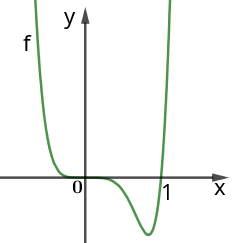
\includegraphics[width=0.3\textwidth]{fig_apl_deriv/GrafInfx^26-x^5.png}}\hfill
\subfigure[]{\label{fig:GrafInf(x-3)^2-2}%
 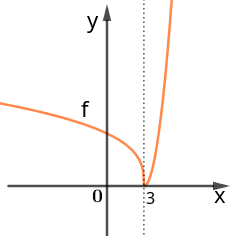
\includegraphics[width=0.3\textwidth]{fig_apl_deriv/GrafInf(x-3)^2-2.png}}\hfill
\subfigure[]{\label{fig:GrafInf(x+1)_(x-5)}%
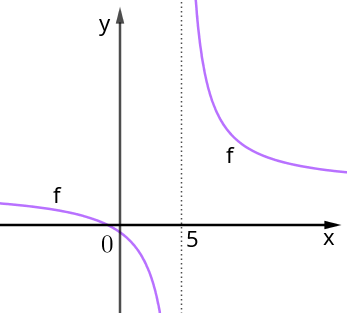
\includegraphics[width=0.35\textwidth]{fig_apl_deriv/GrafInf(x+1)_(x-5).png}}\hfill
\end{figure}

\item \(f(x)=\dfrac{x+1}{x-5}\)

\begin{solution}
\begin{compactenum}[i.]
\item \({\rm Dom}(f)=\mathbb{R}\setminus \{5\}\);
\item \(f\) é contínua em \({\rm Dom}(f)\);
\item Da definição de \(f\), temos que \(f'(x)=- \dfrac{6}{(x-5)^2}\);
\item Da definição de \(f'\), temos que \(f''(x)=\dfrac{12}{(x-5)^3}\);

Note que, \( x=5\) não é um ponto crítico de inflexão, pois \( 5 \notin {\rm Dom}(f)\). Portanto, \(f\) não tem pontos de inflexão, e os intervalos onde analisaremos se \(f\) é côncava para cima ou para baixo são:

\[ (-\infty, 5)\quad \mbox{e} \quad \left(5,+\infty\right). \]
A análise dos sinais de \(f''(x)\) é mostrada na tabela a seguir:
\begin{center}
  \begin{tabular}{l|c|c}
  \toprule
    \textbf{Intervalos} &	\emph{Sinal de \(f''\)} &	\textbf{Concavidade}\\\hline
\((-\infty, 5)\) &\(-\)&para baixo\\\hline
  \((5,+\infty)\) & \(+\) & para cima\\
    \bottomrule
  \end{tabular}
  \end{center}
\end{compactenum}
O item (c) da figura acima mostra o gráfico dessa função.
\end{solution}


\end{compactenum}
\subsection{Teste da segunda derivada}
\begin{framed}
\begin{teo}
Seja $x_0$ um ponto crítico\index{Ponto crítico} de uma dada função $f$ duas vezes diferenciável e $f''$ contínua em um intervalo aberto contendo $x_0$. Temos
\begin{enumerate}[a)]
\item se $f'(x_0) = 0$ e $f''(x_0) > 0$, então $x_0$ é um ponto de \textbf{mínimo}\index{Função!mínimo} local de $f$;
\item se $f'(x_0) = 0$ e $f''(x_0) < 0$, então $x_0$ é um ponto de \textbf{máximo}\index{Função!máximo} local de $f$.
\end{enumerate}
\end{teo}\end{framed}
\begin{ex}
  A função $f(x) = 2x^3 - 9x^2 + 12x - 2$ tem pontos críticos
  \begin{align*}
    f'(x) = 6x^2 - 18x + 12 = 0 &\Rightarrow x^2 - 3x + 2 = 0 \\
                                &\Rightarrow x = \frac{3 \pm \sqrt{1}}{2}\\
                                &\Rightarrow x_1 = 1,\quad x_2 = 2
  \end{align*}
  A segunda derivada de $f$ é
  \begin{equation*}
    f''(x) = 12x - 18
  \end{equation*}
  Logo, como $f''(x_1) = f''(1) = -6 < 0$, temos que $x_1 = 1$ é ponto de máximo\index{Valor!máximo} local de $f$. E, como $f''(x_2) = f''(2) = 6 > 0$, temos que $x_2 = 2$ é ponto de mínimo\index{Valor!mínimo} local de $f$.
\end{ex}

\begin{obs}
  Se $f'(x_0) = 0$ e $f''(x_0) = 0$, então $x=x_0$ pode ser ponto extremo local de $f$ ou não. Ou seja, o teste é inconclusivo.
\end{obs}

\begin{ex}
  Vejamos os seguintes casos:
  \begin{enumerate}[a)]
  \item A função $f(x) = x^3$ tem ponto crítico
    \begin{align*}
      f'(x) = 0 &\Rightarrow 3x^2 = 0 \\
                &\Rightarrow x = 0
    \end{align*}
    Neste ponto, temos
    \begin{equation*}
      f''(x) = 6x \Rightarrow f''(0) = 0
    \end{equation*}
    Neste caso, $x=0$ não é ponto de extremo local e temos $f'(0) = 0$ e $f''(0) = 0$.
  \item A função $f(x) = x^4$ tem um ponto crítico
    \begin{align*}
      f'(x) = 0 &\Rightarrow 4x^3 = 0 \\
                &\Rightarrow x = 0
    \end{align*}
    Neste ponto, temos
    \begin{equation*}
      f''(x) = 12x^2 \Rightarrow f''(0) = 0
    \end{equation*}
    Neste caso, $x=0$ é ponto de mínimo local e temos $f'(0)=0$ e $f''(0) = 0$.
  \end{enumerate}
\end{ex}
\subsection{Exercícios resolvidos}
\begin{exeresol}
  Encontre o valor máximo global de $f(x) = (x-1)e^{-x}$.
\end{exeresol}
\begin{resol}
  Como $f$ é diferenciável em toda parte, temos que seu valor máximo (se existir) ocorre em ponto crítico tal que
  \begin{align*}
    f'(x) = 0 &\Rightarrow (2-x)e^{-x} = 0 \\
              &\Rightarrow 2-x = 0 \\
              &\Rightarrow x = 2
  \end{align*}
  Agora, usando o teste da segunda derivada, temos
  \begin{align*}
    f''(x) = (x-3)e^{-x} \Rightarrow f''(2) = -e^{-2} < 0
  \end{align*}
  Logo, $x=2$ é ponto de máximo local. O favor da função neste ponto é $f(2) = e^{-2}$. Ainda, temos
  \begin{align*}
    &\lim_{x\to -\infty} (x-1)e^{-x} = -\infty, \\
    &\lim_{x\to \infty} (x-1)e^{-x} = 0
  \end{align*}
  Por tudo isso, concluímos que o valor máximo global de $f$ é $f(2) = e^{-2}$.

\end{resol}

\begin{exeresol}
  Determine e classifique os extremos da função
  \begin{equation*}
    f(x) = x^4 - 4x^3 + 4x^2
  \end{equation*}
  restrita ao intervalo de $[-1, 3]$.
\end{exeresol}
\begin{resol}
  Como $f$ é diferenciável em $(-1, 3)$, temos que seus extremos locais ocorrem nos seguintes pontos críticos
  \begin{align*}
    f'(x) = 0 &\Rightarrow 4x^3-12x^2+8x = 0 \\
              &\Rightarrow 4x(x^2-3x+2)=0 \\
              &\Rightarrow x_1 = 0, x_2 = 1, x_3 = 2
  \end{align*}
  Calculando a segunda derivada de $f$, temos
  \begin{equation*}
    f''(x) = 12x^2 - 24x + 8
  \end{equation*}
  Do teste da segunda derivada, temos
  \begin{align*}
    & f''(x_1) = f''(0) = 8 > 0 \Rightarrow x_1=0 ~ \text{pto. mín. local} \\
    & f''(x_2) = f''(1) = -4 < 0 \Rightarrow x_2=1 ~ \text{pto. máx. local} \\
    & f''(x_3) = f''(2) = 8 > 0 \Rightarrow x_3=2 ~ \text{pto. mín. local} 
  \end{align*}
  Agora, vejamos os valores de $f$ em cada ponto de interesse.
  \begin{center}
    \begin{tabular}{l|ccccc}
      $x$     & $-1$ & $0$ & $1$ & $2$ & $3$ \\\hline
      $f(x)$  & $9$    & $0$   & $1$   & $0$ & $9$ \\
    \end{tabular}\\
  \end{center}
  Então, podemos concluir que $x=-1$ e $x=3$ são pontos de máximo global (o valor máximo global é $f(-1)=f(3)=9$), $x=1$ é ponto de máximo local, $x=0$ e $x=2$ são pontos de mínimo global (o valor mínimo global é $f(0)=f(2)=0$).
  
\end{resol}
\subsection{Exercícios}
\begin{exer}
  Use o teste da segunda derivada para encontrar e classificar o(s) ponto(s) extremo(s) de $f(x) = x^2 - 2x$
\end{exer}
\begin{resp}
  $x=1$ ponto de mínimo global
\end{resp}

\begin{exer}
  Use o teste da segunda derivada para encontrar e classificar o(s) ponto(s) extremo(s) de $\displaystyle f(x) = \frac{x^3}{3}-x$.
\end{exer}
\begin{resp}
  $x_1=-1$ ponto de máximo local; $x_2=1$ ponto de mínimo local;
\end{resp}

\begin{exer}
  Use o teste da segunda derivada para encontrar e classificar o(s) ponto(s) extremo(s) de $\displaystyle f(x) = x^{2/3}(x-1)$.
\end{exer}
\begin{resp}
  $x_1=0$ ponto de máximo local; $x_2=2/5$ ponto de mínimo local;
\end{resp}

\begin{exer}
  Seja $f(x) = -x^4$. Mostre que $x=0$ é ponto de máximo local de $f$ e que $f'(0) = f''(0) = 0$.
\end{exer}
\begin{resp}
  $f'(x) = -4x^3$, $f'(0)=0$. Pelo teste da 1ª derivada, temos que $x=0$ é ponto de máximo local. $f''(x) = -12x^2$, $f''(0)=0$.
\end{resp}
\section[\formula{Esboçando o gráfico de uma função $y = f(x)$}]{\boldmat{Esboçando o gráfico de uma função $y = f(x)$}}
O esboço do gráfico de uma função é muito importante, pois com ele podemos determinar o seu
comportamento em R. Para esboçar o gráfico de uma função, precisaremos da teoria de limites, de
continuidade e de derivadas. O procedimento é o seguinte:
\begin{enumerate}[1.]
\item Determinar o domínio de \(f\), \({\rm Dom}(f)\);
\item Determinar as interseções com os eixos;
\item Verificar a simetria da função, a existência de assíntotas, os limites nos extremos de \({\rm Dom}(f)\) e nos pontos de descontinuidade, a fim de determinar o comportamento da função nesses pontos;
\item Determinar os intervalos de crescimento e decrescimento, e os valores extremos da função;
\item Determinar os intervalos de concavidade para cima e para baixo, e os pontos de inflexão;
\item Esboçar o gráfico da função com informações obtidas.
\end{enumerate}

\begin{ex}
Esboce o gráfico de \(f\) definida por:

\begin{enumerate}[a)]
\item \(f(x)=\dfrac{x^2-x-2}{x-5}\)

\begin{solution}
\begin{enumerate}[1.]
\item \({\rm Dom}(f)=\mathbb{R}\setminus\{5\}\);
\item Interseções com os eixos:
\begin{itemize}
    \item Com o eixo \(y\): para \(x=0\), temos que \(f(0)=2/5\)
\item Com o eixo \(x\): para \(f(x)=0\), temos que \(x=-1\) ou \(x=2\)
\end{itemize}
Logo, os pontos de interseção com os eixos são: \((0,2/5)\), \((-1,0)\) e \( (2,0)\).
\item 
\begin{itemize}
    \item O gráfico não é simétrico com respeito ao eixo \(y\) pois \(f(-x)\neq f(x)\)

\item Assíntota vertical: \(x=5\) porque

\[ \lim\limits_{x\to 5^-}f(x)=-\infty\quad \mbox{e}\quad \lim\limits_{x\to 5^+}f(x)=+\infty; \]
\item Assíntotas horizontais: não existem porque

\[ \lim\limits_{x\to-\infty}f(x)=-\infty\quad \mbox{e}\quad \lim\limits_{x\to+\infty}f(x)=+\infty; \]
\item Assíntotas oblíquas: \(y=x+4\) é a única oblíqua porque

\[ \lim\limits_{x\to \pm\infty}\dfrac{f(x)}{x}=1\quad \mbox{e}\quad \lim\limits_{x\to\pm\infty}(f(x)-x)=4. \]
\end{itemize}
\item Da definição de \(f\), temos que \(f'(x)= \dfrac{x^2-10x+7}{(x-5)^2}\).
Logo, os pontos críticos são \(x=5-3\sqrt{2}\) e \(x=5+3\sqrt{2}\), e os intervalos onde analisaremos o crescimento ou decrescimento de \(f\) são:

\[ (-\infty,5-3\sqrt{2} ),\quad (5-3\sqrt{2},5),\quad (5,5+3\sqrt{2})\quad \mbox{e}\quad (5+3\sqrt{2}, +\infty ). \]
A análise dos sinais de \(f'(x)\) é mostrada na tabela a seguir:
\begin{center}
  \begin{tabular}{l|c|c}
  \toprule
    \textbf{Intervalos} &	\emph{Sinal de \(f'\)} &	\textbf{Concavidade}\\\hline
\((-\infty,5-3\sqrt{2} )\) &\(+\)& crescente\\\hline
  \((5-3\sqrt{2},5)\) & \(-\) & decrescente\\\hline
  \((5,5+3\sqrt{2})\) & \(-\) & decrescente\\\hline
  \((5+3\sqrt{2}, +\infty )\) & \(+\) & crescente\\
    \bottomrule
  \end{tabular}
  \end{center}
  Então, \(f(5-3\sqrt{2})\) é um valor máximo e \(f(5+3\sqrt{2})\) é um valor mínimo.
  \item Da definição de \(f'\), temos que \(f''(x)= \dfrac{36}{(x-5)^3}\).
Logo, não existem pontos críticos de inflexão, pois \(5 \notin {\rm Dom}(f)\) e os intervalos onde analisaremos a concavidade para cima ou para baixo de \(f\) são:

\[ (-\infty,5)\quad \mbox{e}\quad (5, +\infty ). \]
A análise dos sinais de \(f''(x)\) é mostrada na tabela a seguir:
\begin{center}
  \begin{tabular}{l|c|c}
  \toprule
    \textbf{Intervalos} &	\emph{Sinal de \(f''\)} &	\textbf{Concavidade}\\\hline
\((-\infty,5 )\)&\(-\)& para baixo\\\hline
  \((5-3\sqrt{2},5)\) & \(-\) & para baixo\\\hline
  \((5, +\infty )\) & \(+\) & para cima\\
    \bottomrule
  \end{tabular}
  \end{center}
  \item Portanto, o gráfico de \(f\) é o item (a) da figura a seguir:
  \begin{figure}[H]
    \centering
    \subfigure[]{\label{fig:Grafy=f(x)-(x^2-x-2)_(x-5)}%
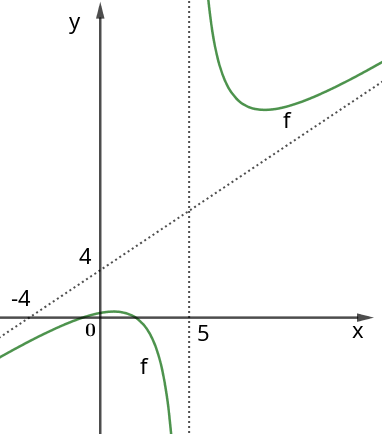
\includegraphics[width=0.35\textwidth]{4-cap_apl_derivadas/fig_apl_deriv/Grafy=f(x)-(x^2-x-2)_(x-5).png}}\quad
\subfigure[]{\label{fig:Grafy=f(x)-x_(x-2)}%
 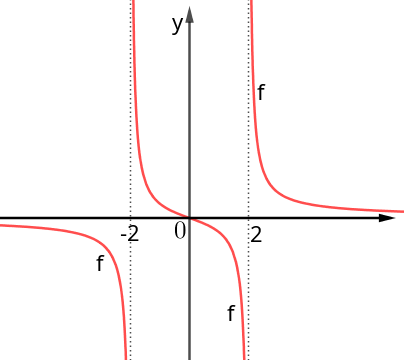
\includegraphics[width=0.42\textwidth]{4-cap_apl_derivadas/fig_apl_deriv/Grafy=f(x)-x_(x-2).png}}
\end{figure}
\end{enumerate}
\end{solution}
\item \(f(x)=\dfrac{x}{x^2-4}\)

\begin{solution}
\begin{enumerate}[1.]
    \item \({\rm Dom}(f)=\mathbb{R}\setminus \{-2,2\}\);
    \item Interseções com os eixos: \((0,0)\);
    \item 
    \begin{itemize}
        \item O gráfico de \(f\) não é simétrico em relação ao eixo \(y\) porque \(f(-x)\neq f(x)\).
        \item Assíntotas verticais: \(x=-2\) e \(x=2\), porque

\[ \lim\limits_{x\to -2^-}f(x)=-\infty\quad \mbox{e}\quad \lim\limits_{x\to -2^+}f(x)=+\infty; \] \[ \lim\limits_{x\to 2^-}f(x)=-\infty\quad \mbox{e}\quad \lim\limits_{x\to 2^+}f(x)=+\infty; \]
\item Assíntota horizontal: \(y=0\);
\item Assíntotas oblíquas: não existem.
    \end{itemize}

\item Da definição de \(f\), temos que \(f'(x)= -\dfrac{x^2+4}{(x^2-4)^2}\).
Logo, não existem pontos críticos, e os intervalos onde analisaremos o crescimento ou decrescimento de \(f\) são:

\[ (-\infty,-2 ),\quad (-2,2)\quad \mbox{e}\quad (2, +\infty ). \]
Porém, neste caso não será necessário fazer este analise, já que, \(f'(x)<0\) para todo \(x \in {\rm Dom}(f)\). Assim, \(f\) é decrescente em \({\rm Dom}(f)\).
\item Da definição de \(f'\), temos que \(f''(x)= \dfrac{2x(x^2+12)}{(x^2-4)^3}\).
Logo, \(x=0\) é um ponto crítico de inflexão, e os intervalos onde analisaremos a concavidade para cima ou para baixo de \(f\) são:

\[ (-\infty,-2 ),\quad (-2,0),\quad (0,2)\quad \mbox{e}\quad (2, +\infty ). \]
A análise dos sinais de \(f''(x)\) é mostrada na tabela a seguir:
\begin{center}
  \begin{tabular}{l|c|c}
  \toprule
    \textbf{Intervalos} &	\emph{Sinal de \(f''\)} &	\textbf{Concavidade}\\\hline
\((-\infty,-2 )\)&\(-\)& para baixo\\\hline
  \((-2,0)\)& \(+\) & para cima\\\hline
  \((0,2)\) & \(-\) & para baixo\\\hline
  \((2, +\infty )\) & \(+\) & para cima\\
    \bottomrule
  \end{tabular}
  \end{center}
  Assim, para \(x=0\), temos que o ponto \(P=(0,f(0))=(0,0)\) é um ponto de inflexão;
  \item Portanto, o gráfico de \(f\) é o item (b) da figura acima.
\end{enumerate}
\end{solution}
\end{enumerate}


\end{ex}



\section{Taxas de Variação}\hypertarget{TaxaVar}{}\label{sec:taxaVariac}
De uma forma geral, se $y = f ( x )$ é uma função, a razão $\frac{\Delta y}{\Delta y}$ é chamada de \textbf{taxa média de variação} da função $f$ no intervalo $[ x, x + \Delta x ]$ e a derivada $$f'(x)=\lim_{\Delta x\to 0}\frac{f(x+\Delta x)-f(x)}{\Delta x}$$ é chamada de \textbf{taxa de variação} da função $f$ no ponto $x$.
\begin{center}
   \textbf{ “Toda taxa de variação pode ser interpretada como uma derivada”.}
\end{center}


Interpretando a derivada desta forma, podemos resolver diversos problemas das ciências que 
envolvem razões instantâneas de variação. 
\begin{ex}
 Suponha que um óleo derramado através da ruptura do tanque de um navio se espalhe em forma circular cujo raio cresce a uma taxa de $2\, m/h$. Com que velocidade a área do derramamento está crescendo no instante em que o raio atingir $60\, m$?\\
 \textbf{Solução:}\\
 A taxa com que o raio cresce é de $2\, m/h$. Podemos interpretar e denotar esta taxa de variação como $$\frac{dr}{dt}=2\, m/h$$
 
Queremos calcular a taxa com que a área cresce em relação ao tempo. Podemos denotar esta taxa de variação como $\frac{dA}{dt}$. A área do derramamento é circular, logo $$A = \pi r^2$$ 

Queremos calcular $\frac{dA}{dt}$  e temos $\frac{dr}{dt}$. A \textbf{regra da cadeia} relaciona estas razões através de 
\matt{ \frac{dA}{dt}=\frac{dA}{dr}\cdot \frac{dr}{dt}
}
Assim,
\matt{
\frac{dA}{dt}=2\pi r\cdot 2=4\pi r
}

Quando o raio atingir $60\, m$ a área do derramamento  estará crescendo a uma taxa de $4\pi (60)\,  m^2/h=240\pi\, m^2/h$.
\end{ex}
\subsection{\hspace{-0.3cm}Diretrizes para resolver problemas de taxa de variação}
\begin{enumerate}[1.]
\item  Desenhe uma figura para auxiliar a interpretação do problema; 
\item Identifique e denote as taxas que são conhecidas e a que será calculada; 
\item  Ache uma equação que relacione a quantidade, cuja taxa será encontrada, com as quantidades 
 cujas taxas são conhecidas; 
\item Derive esta equação em relação ao tempo, ou use a regra da cadeia, ou a derivação implícita 
 para determinar a taxa desconhecida; 
\item Após determinada a taxa desconhecida, calcule-a em um ponto apropriado. 
\end{enumerate}
\hrule
\begin{ex}
Um tanque de água tem a forma de um cone circular invertido com base de raio $2\, m$ e altura igual a $4 \, m$. Se a água está sendo bombeada dentro do tanque a uma taxa de $2 \, m^3/min$, encontre  a taxa na qual o nível da água está elevando quando a água está a $3\, m$ de profundidade.\\
\textbf{Solução:}\\

   Dado $\frac{dV}{dt}=2 \, m^3/min$, devemos encontrar $\frac{dh}{dt}$ quando $h = 3\, m$. As grandezas $V$ e $h$ estão relacionadas pela equação do volume do cone: $$V=\frac{1}{3}\pi r^2 h$$
    \begin{minipage}{0.45\textwidth} 
    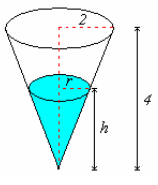
\includegraphics[width=4.5cm]{fig_apl_deriv/tanquecone.png}
    \end{minipage}
\hfill
 \begin{minipage}{0.55\textwidth} 
 Para obter o volume $V$ como função 
da altura $h$, podemos ``eliminar'' a variável $r$ usando semelhança de triângulos: 
$$\frac{r}{h}=\frac{2}{4}\Rightarrow r=\frac{h}{2}$$

Assim $V=\frac{1}{3}\pi\pc{\frac{h}{2}}^2h=\frac{\pi}{12}h^3$
    \end{minipage}

Derivando ambos os lados em relação ao tempo $t$, obtemos 
\matt{
\frac{dV}{dt}=\frac{dV}{dh}\cdot \frac{dh}{dt}\Leftrightarrow \frac{dV}{dt}=\frac{\pi}{12}3h^2\frac{dh}{dt}\Leftrightarrow\frac{dh}{dt}=\frac{4}{\pi h^2}\cdot \frac{dV}{dt}
}
Substituindo $\frac{dV}{dt}=2\, m^3/min$ e $h=3\, m$, temos
\matt{
\frac{dh}{dt}=\frac{4}{\pi 3^2}\cdot 2=\frac{8}{9\pi}\approx 0,28\, m/min.
}
\end{ex}
\subsection{Exercícios}
\begin{exer}
Uma bola de neve esférica é formada de tal maneira que o seu volume aumenta à razão de $8  \, cm^3/min$. Com que velocidade aumenta o raio no instante em que a bola tem $4   \, cm$ de diâmetro? 
\end{exer}
\begin{exer}
 Um automóvel que viaja à razão de $30   \, m/s$, aproxima-se de um cruzamento. Quando o automóvel está a $120\, m$ do cruzamento, um caminhão que viaja à razão de $40  \, m/s$ atravessa o cruzamento. O automóvel e o caminhão estão em rodovias que formam um ângulo reto uma com a outra. Com que velocidade afastam-se o automóvel e o caminhão $2\,s$ depois do caminhão passar pelo cruzamento? 
\end{exer}
\begin{exer}
 Uma escada com $13\, m$ de comprimento está apoiada numa parede vertical e alta. Num determinado instante a extremidade inferior, que se encontra a $5\, m$ da parede, está escorregando, afastando-se da parede a uma velocidade de $2   \, m/s$. Com que velocidade o topo da escada está deslizando neste momento? 
\end{exer}
\begin{exer}
Um balão está a $60\, m $ acima do solo e se eleva verticalmente à razão de $5   \, m/s$. Um automóvel  passa por baixo do balão viajando à $12   \, m/s$. Com que velocidade varia, um segundo depois, a distância entre o balão e o automóvel? 
\end{exer}
\begin{exer}
 Despeja-se água num recipiente de forma cônica, à razão de $8   \, cm^3/min$. O cone tem $20   \, cm $ de profundidade e $10   \, cm$ de diâmetro em sua parte superior. Se existe um furo na base, e o nível da água está subindo à razão de $1\, mm/min$, com que velocidade a água estará escoando quando esta estiver a $16   \, cm$ do fundo? 
\end{exer}
\begin{exer}
Um lado de retângulo está crescendo a uma taxa de $17   \, cm/min$ e o outro lado está decrescendo a uma taxa de $5   \, cm/min$. Num certo instante, os comprimentos desses lados são $10   \, cm $ e $ 7   \, cm$, respectivamente. A área do retângulo está crescendo ou decrescendo nesse instante? A que velocidade? 
\end{exer}
\begin{exer}
Dois resistores variáveis $R_1 $ e $R_2$  são ligados em paralelo. A resistência total $R$ é calculada 
pela equação $\frac{1}{R}=\frac{1}{R_1}+\frac{1}{R_2}$. Se $R_1$ e $ R_2$  estão aumentando às taxas de 
$0,01\, ohm/s$ e $0,02\, ohm/s$ respectivamente, a que taxa varia $R$ no instante em que $R_1= 30\, ohm/s$ e $R_2= 90\, ohm/s$?
\end{exer}
\begin{exer}
Um triângulo isósceles tem os lados iguais com $15   \, cm$ cada um. Se o ângulo $\theta $ entre eles varia à 
razão de $\pi /90\, rad$ por minuto, determine a variação da área do triângulo quando $\theta  = \pi/6 \, rad$. 
\end{exer}
%************************************************************************************
\section{Problemas de otimização}\hypertarget{Otimiza}{}\label{sec:Otmiz}
 Agora apresentaremos os problemas de otimização. Nestes problemas buscamos soluções que são ótimas, do ponto de vista matemático. Por exemplo: uma empresa deseja produzir potes cilíndricos de $300\, ml$ para armazenar certo tipo de produto. Sabe-se que estes potes devem ter  área total mínima para reduzir o custo de impressão dos rótulos. De todos os cilindros de volume igual a $300\; ml$, qual possui menor área total (raio da base e altura)? Devemos então buscar uma solução que minimize a área total do cilindro, reduzindo assim o custo de impressão dos rótulos nos potes. Variados problemas práticos, semelhantes a esse, em diversos ramos do conhecimento, são resolvidos com o auxílio das derivadas. 

Iniciaremos resolvendo este problema. 
\vspace{0.5cm}
\begin{ex}
De todos os cilindros de volume igual a $300\, ml$, qual possui menor área total (raio da base e altura)?\\
\textbf{Solução:}

Abrindo o cilindro nós temos 
\begin{figure}[H]
    \centering
    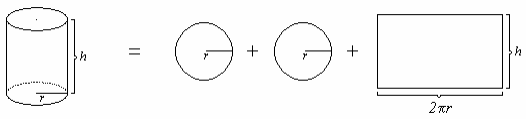
\includegraphics{fig_apl_deriv/Cilindro-Planif.png}
    \end{figure}
    
    Sabe-se que o volume do cilindro é $V=\pi r^2h$ e a área total é $A=2\pi r^2+2\pi rh$. 
    
Queremos determinar os valores do raio ($r$) da base e a altura ($h$) de um cilindro de $300 \, ml$ de volume ($V$) que possua mínima área total ($A$).

Já sabemos determinar o ponto de mínimo de uma função através dos dois critérios vistos, mas a função área possui duas variáveis $r$ e $h$. Poderemos resolver este problema isolando uma das variáveis em $V=\pi r^2h$ (com $V = 300$) e substituí-la em $A=2\pi r^2+2\pi rh$.
\matt{
300=\pi r^2h\Rightarrow h=\frac{300}{\pi r^2}
}
Temos então que $$A=2\pi r^2+2\pi r\frac{300}{\pi r^2}=2\pi r^2+\frac{600}{r}$$

Conseguimos então tornar a função área como função de uma única variável. Vamos determinar o ponto crítico desta função:\\ 
$$A'=4\pi r-\frac{600}{r^2}$$
Resolvendo agora a equação $A'=0$:
$$4\pi r-\frac{600}{r^2}=0\Rightarrow 4\pi r=\frac{600}{r^2}\Rightarrow r=\sqrt[3]{\frac{600}{4\pi}}=\approx 3,6\, cm$$
Como $A''\pc{\sqrt[3]{\frac{600}{4\pi}}}>0$ (Verifique!), temos que $r=\sqrt[3]{\frac{600}{4\pi}}$ é ponto de mínimo da função $A$ (pelo critério da segunda derivada). Substituindo $r=\sqrt[3]{\frac{600}{4\pi}}$  em $h=\frac{300}{\pi r^2}$, obtemos $h\approx 7,2\; cm$.
\end{ex}
\subsection{\hspace{-0.3cm}Diretrizes para resolução de problemas de otimização}
 \begin{enumerate}
\item Leia cuidadosamente o problema. Esboce uma figura para auxiliar a sua interpretação; 
\item Identifique e denomine com variáveis as quantidades informadas no problema; 
\item  Determine algumas relações (ou fórmulas) entre as variáveis; 
\item  Determine qual variável deve ser otimizada (maximizada ou minimizada). Expresse esta variável como função de uma das outras variáveis; 
\item Determine o ponto crítico da função obtida o item anterior; 
\item Determine o(s) extremo(s) com o auxílio dos critérios da 1ª  e 2ª derivadas. 
\end{enumerate}
\begin{ex}
 Determine as dimensões (base e altura) do retângulo de área máxima que pode ser 
inscrito em um semicírculo de raio constante a, como mostra a figura. 
\begin{figure}[H]
    \centering
    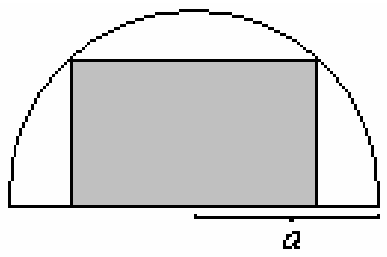
\includegraphics[scale=0.9]{fig_apl_deriv/RetInSemiCirc.png}
    \end{figure}
\end{ex}
Podemos dizer que este retângulo tem base igual a $b$ e altura igual a $h$. Observe a figura abaixo, onde $a$ é o raio do semicírculo.  
\begin{figure}[H]
    \centering
    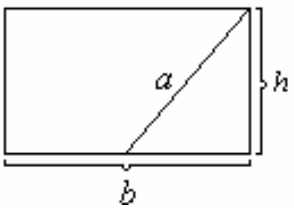
\includegraphics{fig_apl_deriv/RetInSemiCirc2.png}
    \end{figure}
Queremos maximizar a área do retângulo $A = bh$, sabendo-se que as variáveis b e h obedecem o 
teorema de Pitágoras $$\pc{\frac{b}{e}}^2+h^2=a^2$$
Isolando a a variável $h$, temos
$$h=\sqrt{a^2-\pc{\frac{b}{2}}^2}=\frac{\sqrt{4a^2-b^2}}{2}$$
Podemos então tornar a função área como função de uma única variável $b$ (Lembre-se que a é uma constante!), pois 
$$A=b\cdot\frac{\sqrt{4a^2-b^2}}{2}=\frac{1}{2}\cdot b\frac{\sqrt{4a^2-b^2}}{2} $$
Resolvendo a equação $A'( b) = 0$ , obtemos: 
$$A'=\frac{1}{2}\sqrt{4a^2-b^2}+\frac{b}{2}\cdot\frac{-2b}{2\sqrt{4a^2-b^2}}=\frac{\sqrt{4a^2-b^2}}{2}-\frac{b^2}{2\sqrt{4a^2-b^2}}$$
$$A'=0\Leftrightarrow\frac{\sqrt{4a^2-b^2}}{2}=\frac{b^2}{2\sqrt{4a^2-b^2}}\Leftrightarrow 4a^2-b^2=b^2\Leftrightarrow 2b^2=4a^2\Leftrightarrow \boldsymbol{b=a\sqrt{2} }$$
Substituindo $\boldsymbol{b=a\sqrt{2} } $ em $h=\frac{\sqrt{4a^2-b^2}}{2}$, obtemos $\boldsymbol{h=\frac{a\sqrt{2}}{2}}$\\
Verifique que realmente $\boldsymbol{b=a\sqrt{2} } $ é o ponto de máximo da função área $A=\frac{b\sqrt{4a^2- b^2}}{2}$ usando  o critério da segunda derivada $A''(a\sqrt{2})<0$.
\subsection{Exercícios}
\begin{exer}
 De todos os retângulos de comprimento fixo $L$, qual possui maior área? Determine a base e a 
altura de tal retângulo.
\end{exer}
\begin{exer}
 Uma reta variável passando por $P (1, 2)$ corta o eixo $Ox$ em $A(a,0)$ e o eixo $Oy$ em $B(b,0)$. Determine o triângulo $OAB$ de área mínima, para $a$ e $b$ positivos. 
 \end{exer}
 \begin{exer}
 Uma fábrica produz $x$ milhares de unidades mensais de um determinado artigo. Se o custo de produção é dado por $C(x)=2x^3+6x^2+18x+6$ e a receita obtida na venda é dada por $R(x)=60-12x^2$, determinar o número ótimo de unidades que maximiza o lucro $L$. Obs.: $Lucro = Receita - Custo$, isto é, $L(x)=R(x)-C(x)$.
 \end{exer}
  \begin{exer}
Usando uma folha quadrada de cartolina, de lado igual a $60\, cm$, deseja-se construir uma caixa  sem tampa, cortando seus cantos em quadrados iguais e dobrando convenientemente a parte restante. Determinar o lado dos quadrados que devem ser cortados de modo que o volume da caixa seja o maior possível.
\begin{figure}[H]
    \centering
    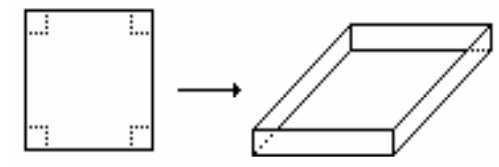
\includegraphics{fig_apl_deriv/Otmiz-PlanifCaixa.png}
\end{figure}
\end{exer}
\begin{exer}
 Corta-se um pedaço de arame de comprimento L em duas partes. Com uma das partes faz-se uma circunferência e com a outra um quadrado. Determine o raio da circunferência e o lado do quadrado para que a soma das áreas compreendidas pelas duas figuras seja mínima. 
 \end{exer}
\begin{exer}
Um construtor deseja construir um depósito com as seguintes características: capacidade de $30 \, m^3$, teto plano, base retangular cuja largura é três quartos do comprimento. O custo por metro quadrado do material é de R\$ 36,00 para o chão, R\$ 204,00 para os lados e R\$ 102,00 para o teto. Quais as dimensões do depósito que minimizarão o custo? 
\end{exer}
\begin{exer}
Dentre os retângulos com base no eixo $Ox$ e vértices superiores sobre a parábola $y = 12 - x^2$ , determine o de área máxima (base e altura). 
\begin{figure}[H]
    \centering
    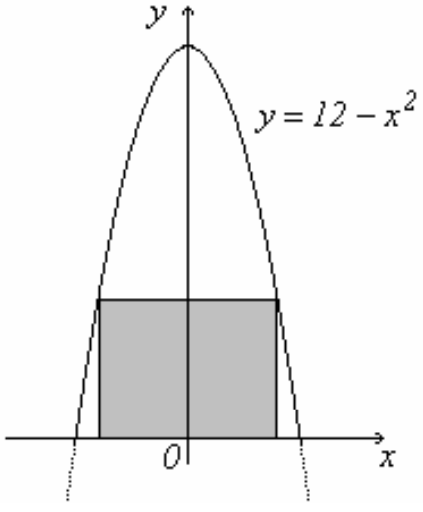
\includegraphics[scale=0.55]{fig_apl_deriv/Otmiz-ParabAreaRet.png}
    \end{figure}
\end{exer}
\begin{exer}
 A potência $P$ de uma bateria de um automóvel é dada por $P = V I - I^2 R$, sendo $I$ a corrente para uma voltagem $V$ e resistência interna da bateria $R$. São constantes $V$ e $R$. Que corrente corresponde à potência máxima?
 \end{exer}
\begin{exer}
O departamento de trânsito de uma cidade, depois de uma pesquisa, constatou que num dia normal da semana à tarde, entre 2 e 7 horas, a velocidade do tráfego é de aproximadamente $V(t)=2t^3-27t^2+108t-35$ quilômetros por hora, onde $t $ é o número de horas transcorridas após o meio dia. A que horas do intervalo de 2 às 7 o tráfego flui mais rapidamente e a que horas flui mais  lentamente, e com que velocidade? 
\end{exer}
\begin{exer}
 Faz-se girar um triângulo retângulo de hipotenusa dada $H$ em torno de um de seus catetos, gerando um cone circular reto. Determine o cone de volume máximo (raio da base e altura). 
 \end{exer}
\begin{exer}
Um gerador de corrente elétrica tem uma força eletromotriz de $\epsilon$ volts e uma resistência interna de $r\, ohms$. $\epsilon$ e $r$ são constantes. Se $R\, ohms$ é uma resistência externa, a resistência total é $(r + R)\,
ohms$ e se $P\, watts$ é a potência então, $P=(\epsilon^2R)/(r+R)^2$. Qual o valor de R que consumirá o máximo
de potência? Interprete o resultado. 
\end{exer}


\section{Recapitulando}
Neste capítulo, apresentamos algumas aplicações da derivada. Começamos entendendo como  as derivadas nos auxiliam também no cálculo de limites indeterminados como, por exemplo \(\dfrac{0}{0}\) ou \(\dfrac{\infty}{\infty}\), entre outros. Para encontrar os valores desses limites recorremos à \hyperlink{Lopital}{Regra de L’Hôpital}.

Não obstante, introduzimos o conceito de \hyperlink{Diff}{diferencial} e aplicamos para aproximar valores de funções. Este conceito será muito útil mais na frente no Curso de Cálculo.

Entendemos como a derivada nos ajuda a estabelecer se uma função está \hyperlink{unc-CrescDecresc}{crescendo ou decrescendo} em um intervalo dado. Aprendemos os conceitos de \hyperlink{MaxMin}{máximo e mínimo, absolutos ou relativos}.

Aplicamos os conceitos de derivadas para entender  que a derivada por si própria é uma função, ela pode ser derivável caso satisfaça certas condições. Assim, as derivadas de ordem superior também nos auxiliam a entender mais ainda o comportamento de uma função, caso elas existam. Especificamente, com a ajuda da segunda derivada, podemos encontrar os pontos de inflexão de uma curva dada e saber se ela é côncava para cima ou para baixo. Novamente, o domínio desse conceito é fundamental, pois nos auxilia no esboço de gráficos de funções.

Também foram apresentados teoremas de suma importância para a compreensão dos conceitos de máximo e mínimo, entre eles, o \hyperlink{TeoValorMedio}{Teorema do Valor Médio}.

Por fim, apresentamos aplicações das derivadas em problemas de \hyperlink{TaxaVar}{taxa de variação} e \hyperlink{Otimiza}{otimização}.

No próximo capítulo, apresentaremos a integral indefinida, que pode ser vista como a operação inversa da derivada, chamada de antiderivada ou primitiva.

 





\end{document}
